\documentclass[10pt,dvips,twoside,reqno]{amsart} 
\usepackage{epsfig}
\usepackage[authoryear]{natbib} \setlength{\oddsidemargin}{0in}
\setlength{\evensidemargin}{0in} \setlength{\topmargin}{-0.25in}
\setlength{\headheight}{0.1in} \setlength{\headsep}{0.15in}
\setlength{\topskip}{0in} \setlength{\footskip}{0.15in}
\setlength{\textwidth}{6.5in} \setlength{\textheight}{9in}

%differential operators
\newcommand{\grad}{\nabla}
\newcommand{\deld}{\nabla \cdot}
\newcommand{\lap}{\Delta}
%boldface in math mode
\newcommand{\bm}[1]{\mbox{{\boldmath ${#1}$}}}
% vectors and tensors
\renewcommand{\vec}[1]{{\bf #1}}
\newcommand{\gvec}[1]{\mbox{{\boldmath ${#1}$}}}
\newcommand{\ten}[1]{\bar{\bm{#1}}}
%derivatives
\newcommand{\od}[2]{\frac{d {#1}}{d {#2}}}
\newcommand{\ods}[2]{\frac{d^2{#1}}{d {{#2}^2}}}
\newcommand{\pd}[2]{\frac{\partial {#1}}{\partial {#2}}}
\newcommand{\pds}[2]{\frac{\partial^2{#1}}{\partial {{#2}^2}}}
\newcommand{\pdsm}[3]{\frac{\partial^2{#1}}{\partial {#2}\,\partial {#3}}}
%funtional analysis
\newcommand{\abs}[1]{\left| #1 \right|}
\newcommand{\norm}[1]{\left\| #1 \right\|}
\newcommand{\iprod}[2]{\left( #1, #2 \right)}
\newcommand{\dprod}[2]{\left\langle #1, #2 \right\rangle}
%real numbers
\newcommand{\field}[1]{\mathbb{#1}}
\newcommand{\R}{\field{R}}
%funciton spaces
\newcommand{\M}{\mathcal{M}}
%delimiters
\newcommand{\pl}{\left(}
\newcommand{\pr}{\right)}
\newcommand{\sbl}{\left[}
\newcommand{\sbr}{\right]}
\newcommand{\dbl}{\left[\hspace{-0.05cm}\left[}
\newcommand{\dbr}{\right]\hspace{-0.05cm}\right]}
\newcommand{\cbl}{\left\{ }
\newcommand{\cbr}{\right\} }
\newcommand{\eqn}[1]{equation \ref {eq:#1}} 
\newcommand{\Eqn}[1]{Equation \ref {eq:#1}} 
\newcommand{\eqnst}[2]{equations \ref{eq:#1} and \ref{eq:#2}} 
\newcommand{\Eqnst}[2]{Equations \ref{eq:#1} and \ref{eq:#2}} 
\newcommand{\eqns}[2]{equations \ref{eq:#1}--\ref{eq:#2}} 
\newcommand{\Eqns}[2]{Equations \ref{eq:#1}--\ref{eq:#2}}
\newcommand{\msection}[1]{ \vspace{.2in} {\noindent \bf #1}.}
\renewcommand{\for}{\mbox{for}\quad}
%\newcommand{\for}{\mbox{for}\quad}
\newcommand{\argmin}{\mbox{argmin}}
\newcommand{\argmax}{\mbox{argmax}}
\newcommand{\fig}[1]{figure \ref{fig:#1}} 
\newcommand{\Fig}[1]{Figure \ref{fig:#1}} 
\newcommand{\figst}[2]{figures \ref {fig:#1} and \ref {fig:#2}} 
\newcommand{\Figst}[2]{Figures \ref {fig:#1} and \ref {fig:#2}} 
\newcommand{\figs}[2]{figures \ref{fig:#1}--\ref{fig:#2}} 
\newcommand{\Figs}[2]{Figures \ref{fig:#1}--\ref{fig:#2}}
\newcommand{\tab}[1]{table \ref {tab:#1}} 
\newcommand{\Tab}[1]{Table \ref {tab:#1}} 
\newcommand{\tabst}[2]{tables \ref {tab:#1} and \ref {tab:#2}} 
\newcommand{\Tabst}[2]{Tables \ref {tab:#1} and \ref {tab:#2}} 
\newcommand{\tabs}[2]{tables \ref{tab:#1}--\ref{tab:#2}} 
\newcommand{\Tabs}[2]{Tables \ref{tab:#1}--\ref{tab:#2}}
\newtheorem{theorem}{Theorem}
\newenvironment{neqnarray}[1]{\begin{minipage}[t]{6.5in}  \begin{minipage}[b]{1.0in} #1 \end{minipage}  \begin{minipage}[b]{5.5in}\begin{eqnarray}}{\end{eqnarray}\end{minipage}\end{minipage}}
\newcommand{\bneqnarray}[2]{\\ \\ \fbox{\begin{neqnarray}{#1} #2 \end{neqnarray}}\\ \\ \noindent} 

\begin{document}

\begin{center}
{\bf NOTES ON FLOW AND TRANSPORT IN POROUS MEDIA \\}
Chris Kees\\
Center for Research in Scientific Computation, Department of Mathematics, North Carolina State University, Raleigh, NC 27695-8205, email: \texttt{chris\_kees@ncsu.edu} \\
December 14, 2004
\end{center}
\markboth{FLOW AND TRANSPORT IN POROUS MEDIA/KEES}{FLOW AND TRANSPORT IN POROUS MEDIA/KEES}

\tableofcontents 

\section{Single Phase Flow}

\subsection{Model Equations}
If only one fluid phase occupies the porous medium then the model is
\begin{eqnarray}
\pd{(\omega \rho)}{t} + \deld (\rho \vec v) + c&=& d \label{eq:mass_balance} \\
\vec v &=& - \frac{\ten{k}_i}{\mu}(\grad p - \rho \vec g) \label{eq:volume_flux} \\
\ten{k}_i &=&  \ten{k}(\vec x) \\
\omega &=& \omega(\vec x,p) \\
\rho &=& \rho(p) \\
\mu &=& \mu(p) 
\end{eqnarray}
\Eqn{mass_balance} is the mass balance. \Eqn{volume_flux}, Darcy's
law, can be derived from a momentum balance if inertia of the fluid is
neglected. The proportionality constant depends on the fluid through
the viscosity, $\mu_w$, and through the medium permeability,
$\ten{k}_i$.  The porosity, $\omega$, is the volumetric fraction of
the porous medium that can transmit fluid. It is usually assumed to be
a (spatially variable) constant or a weakly nonlinear function of
pressure. The density, $\rho $, is the mass of water per unit volume
of water, also usually assumed to be constant or a weakly nonlinear
function of the pressure. The Darcy velocity, $\vec v $, is the
velocity such that the volumetric flux (flow) through a surface with
area $dA$ with unit normal $\gvec \nu$ is $\vec v \cdot \gvec \nu dA$
\citep{Chavent_Jaffre_86}. The sources and sinks are represented by
$c$ and $d$ respectively.  Since the domain is not entirely open to
flow due to the presence of the solid matrix, the Darcy velocity is
sometimes called the filtration velocity, the macroscopic apparent
velocity, or a fictitious velocity (c.f.
\citep{DeMarsily_86,Chavent_Jaffre_86}).  Another relevant velocity is
$\vec v / \omega$, which is the average fluid velocity in the pores,
sometimes called the microscopic velocity or fictitious mean pore
velocity. The intrinsic permeability of the medium, $\ten{k}_i$, is
the part of the proportionality constant in Darcy's law that reflects
the flow properties of the medium (the porosity and the connectivity
of the pore space).  The pressure is $p$ and the gravitational
acceleration vector is $\vec g$. The fluid viscosity, $\mu$, is the
dynamic viscosity of the fluid. Technically all of these quantities
are porous medium-scale quantities, which means that they are different
from their counterparts in classical fluid dynamics in that they are
obtained from some upscaling procedure such as volume averaging.
Furthermore, all of the media properties are usually functions of
space, and $\ten{k}_i$ is usually anisotropic.

\subsubsection{Closure Relations}

Density and porosity equations are often based on their coefficients
of compressibility at a reference pressure $p_0$:
\begin{eqnarray}
  \label{eq:compressibility}
  \beta_f &=& \pl \frac{1}{\rho}\pd{\rho}{p}\pr_{p_0} = \pl \pd{\log(\rho)}{p} \pr_{p_0} \\
  \beta_m &=& \pl \frac{1}{\omega}\pd{\omega}{p}\pr_{p_0} = \pl \pd{\log(\omega)}{p} \pr_{p_0}
\end{eqnarray}
Exponential constitutive laws can be written as
\begin{eqnarray}
\label{eq:expDensity}
\rho(p) &=& \rho_0 e^{\beta_f(p - p_0)} \\
\label{eq:expPorosity}
\omega(\vec x, p) &=& \omega_0(\vec x) e^{\beta_m (p - p_0)} 
\end{eqnarray}
Typically $\beta_f,\beta_m << 1$ so that first order Taylor
series approximations about $p_0$ are accurate:
\begin{eqnarray}
\label{eq:linearDensity}
\rho(p) &=& \rho_0 \pl 1 + \beta_f p \pr \\
\label{eq:linearPorosity}
\omega(\vec x,p) &=& \omega_0(\vec x) \pl 1 + \beta_m p \pr 
\end{eqnarray}
We note that $\omega(p)$ is more complex than $\rho(p)$ in that it
incorporates compressibility of the solid as well as other effects
such as rearrangement of the pore structure. To be consistent these
effects would also need to be represented with a nonlinear
permeability $\ten k_i$, but in practice the simple linear expression
above is used.

For gases, density relations based on ideal or real gases can be used
such as \citep{Helmig_97}
\begin{equation}
  \label{eq:gasDensity}
  \rho = \frac{p-p_0}{Z R T}
\end{equation}
where $Z$ is the real gas factor, $R$ is the gas constant, and $T$ is
the temperature.

\subsection{Working Formulations}

\subsubsection{Dimensionless Variables \label{onePhaseDimensionless}}
The dimensions of the variables are
\begin{center}
\begin{tabular}{ccccccc}
$\omega [-]$ & $\rho [ML^{-3}]$ & $\vec v [LT^{-1}]$ & $\ten{k}_i [L^2]$ & $\mu_w [ML^{-1}T^{-1}]$ &$p [ML^{-1}T^{-2}]$&$\vec g [LT^{-2}]$
\end{tabular}
\end{center}
Let $p_0$ be some reference pressure, say atmospheric pressure, and
$\vec x_0$ be a reference coordinate, say the lowest point in the
domain in some coordinate system. The rank of the dimensional matrix
is 3, which means we can put the equation in dimensionless form with
the choice of three reference scales. We will use a reference length
$l$, the magnitude of gravitational acceleration, $g = \| g\|$, and a
reference density $\rho_0 = \rho(p_0)$. This yields the following
dimensionless variables:
\begin{eqnarray}
\tilde{t} &=& t \sqrt{\frac{g}{l}} \\
\tilde{\vec x} &=& \vec x \frac{1}{l} \\
\tilde{\psi} &=& \frac{p - p_0}{\rho_0 g l} \label{eq:head}\\
\tilde{\rho} &=& \frac{\rho}{\rho_0} \\
\tilde{\ten K} &=& \frac{\rho_0 g \ten k}{\mu \sqrt{gl}} \\
\tilde{\vec v} &=& \vec v \frac{1}{\sqrt{gl}} \\
\tilde{\vec g} &=& \frac{\vec g}{g} \label{eq:dg} \\
\tilde{z} &=& -\tilde{\vec g} \cdot (\tilde{\vec x} - \tilde{\vec x}_0) \\
\tilde{c} &=& \frac{c}{\rho_0}\sqrt{\frac{l}{g}} \\ 
\tilde{d} &=& \frac{d}{\rho_0}\sqrt{\frac{l}{g}} \\ 
\end{eqnarray}
We will assume that for the remainder of this chapter the variables
are dimensionless unless otherwise stated (we will drop the
tilde's).  After substituting the dimensionless variables into
\eqnst{mass_balance}{volume_flux}, we obtain the general dimensionless
form of the single phase flow equation
\begin{equation}
  \label{eq:satFlowDimensionless}
  \pd{\omega \rho}{t} - \deld \rho \ten K \pl \grad \psi + \rho \grad z \pr + c = d 
\end{equation}



\subsubsection{Potentials}

A trick for rewriting nonlinear diffusion terms
\citep{Kirchoff_1894,Carslaw_Jaeger_59} is to use the fact that $a(u)
\grad u = \grad \phi$ where
\begin{equation}
  \label{eq:kirch}
  \phi = \int_{u_0}^{u} a(w) dw
\end{equation}
We can define a potential
\begin{equation}
  \label{eq:totalHead}
  \phi = \int_0^{\psi} \frac{1}{\rho(w)}dw + z
\end{equation}
so that
\begin{equation}
  \label{eq:totalHeadExp}
  \rho \grad \phi = \rho \pl \frac{1}{\rho} \grad \psi + \grad z \pr = \grad \psi + \rho \grad z
\end{equation}
which in the case of an incompressible fluid is just $\phi = \psi +
z$. Since $\od{\phi}{\psi} > 0$, we can assume the existence of
$\psi(\phi,z)$. This potential is sometimes known as the Hubbert
potential, and, in the incompressible case, it is known as the total
hydraulic head. The single phase model can then be reduced to a nonlinear heat equation for $\phi$, which we write as
\begin{equation}
  \pd{(\omega \rho)}{t} - \deld \rho^2 \ten K \grad \phi + c = d \label{eq:volume_flux_potential} 
\end{equation}
Another useful potential is
\begin{equation}
  \label{eq:totalHead2}
  \phi = \int_0^{\psi}\rho(u) du 
\end{equation}
which yields 
\begin{equation}
\pd{(\omega \rho)}{t} - \deld (\ten{K} \grad \phi + \rho^2 \ten K \grad z) + c= d
\end{equation}

\subsubsection{Incompressible Fluid and Medium}
In this case $\omega$ is a constant and $\rho=1$ (it's dimensionless),
which yields
\begin{equation}
  \label{eq:incompressible}
  \deld \ten{K} \grad \phi +c=d
\end{equation}
with $\phi = \psi + z$.

\subsubsection{Slightly Compressible Fluid}

In dimensionless form \eqnst{linearDensity}{linearPorosity} are
\begin{eqnarray}
  \label{eq:slCompressDimensionless}
  \rho &=& 1 + \beta_f \rho_0 g l = 1 + \epsilon_f \psi \\
  \omega &=& \omega_0(1 + \beta_m \rho_0 g l) = \omega_0(1 + \epsilon_m \psi)
\end{eqnarray}
If we neglect higher order terms in
$\epsilon_f$ and $\epsilon_m$ and spatial gradients of $\rho$ \citep{Chavent_Jaffre_86} we obtain

\begin{equation}
\label{eq:onePhaseSlCompPress}
\omega_0 \pl \epsilon_f + \epsilon_m \pr \pd{\psi}{t} - \deld \ten{K} (\grad \psi + \grad z) + c = d
\end{equation}
Often a specific storage coefficient is defined as
\begin{equation}
  \label{eq:specificStorage}
  S_s = \omega_0 (\hat{\beta}_r + \hat{\beta}_f)
\end{equation}

\subsubsection{The Classical Porous Medium Equation}

In the case of gas $\rho = C \psi^{\gamma}$ ($\gamma = 1$ for ideal
gases and the real gas law given above) so the fully compressible
model above is
\begin{equation}
  \label{eq:pome}
\pd{(\omega C \psi^{\gamma} )}{t} + \deld (C^2 \psi^{2\gamma} \ten K \vec g -\ten K C \grad \psi^{\gamma + 1}) = 0
\end{equation}
which is a form of the classical porous medium equation.

\subsection{Boundary and Initial Conditions}

In field applications usually either the pressure (or pressure head or
total head) is specified or the normal flux is specified at each point
of the boundary. In some applications a mixed (Robin) boundary
condition is specified to simulate various other physical situations
(e.g. river and lake boundaries).
\begin{eqnarray}
\phi &=& \phi_d (t,\vec x) \quad \vec x \in \Gamma^D\\
\vec v \cdot \gvec \nu & = & q_n(t,\vec x) \quad \vec x \in \Gamma^N\\
\alpha_r \sbl \phi - \phi_d(t,\vec x) \sbr + \beta_r \sbl \vec v \cdot \gvec \nu - q_n(t, \vec x) \sbr &=& 0
\quad \vec x \in \Gamma^R
\end{eqnarray}
where $\gvec \nu$ is the outward unit normal on $\Gamma$. Initial
conditions are often taken as a static equilibrium condition, which
yields $\phi(\vec x)=c$. Steady flow initial conditions can also be
specified easily in a homogeneous medium with simple boundary
conditions. In the heterogeneous case or for complex boundary
conditions/geometries we may have to solve the steady state problem
for the initial conditions to the transient problem.

\subsection{Sources and Sinks}

Wells can be specified as ``holes'' in the domain and therefore
represented as boundary conditions or as point sources if the domain is
large enough with respect to the well diameter. Recharge to the
aquifer can be represented through boundary conditions but is often
represented as a spatially distributed source as well.
\begin{center}
\fbox{\begin{minipage}[b]{6.5in}
\subsection{Summary}
Single Phase Flow Equation
\begin{equation}
m_t + \deld \pl \vec f - \ten{a} \grad \phi \pr + c = d \\
\end{equation}
\begin{align}
\intertext{Primitive Form Coefficients}
m &= \omega \rho \\
f &= - \rho^2 \ten{K} \grad z \\
\ten{a} &= \rho \ten{K} \\
\phi &= \psi\\
c,d &= \mbox{problem dependent wells and sources} \\
u &= \phi = \psi\\
\intertext{Potential Form Coefficients}
m &= \omega \rho \\
f &= 0 \\
a &= \rho \ten{K}\\
\phi &= \int_0^\psi \frac{1}{\rho(s)}ds + z, \mbox{ or if incompressible} = \psi + z\\
u &= \psi \mbox{ or } u =\phi \\
\intertext{Density Closure Relations (Dimensionless)}
\rho &= 1 &&\mbox{(constant)}\\
\rho &= e^{\beta_f \psi} &&\mbox{(exponential)}\\
\rho &= 1 + \beta_f \psi &&\mbox{(linear)}\\
\rho &= p/Z(p,T)RT &&\mbox{(real gas,Z=1 for ideal)}\\
\rho &= (\psi/\psi_0)^m e^{\beta_f \psi} &&\mbox{(general)}\\
\intertext{Porosity Closure Relations (Dimensionless)}
\rho &= \omega_0 &&\mbox{(constant)}\\
\rho &= 1 + \beta_m \psi &&\mbox{(linear)}\\
\intertext{Dimesional Quanties (Examples--Source http://www.hbcpnetbase.com)}
\rho_0 &= 997.0 && [kg/m^3] \mbox{ for water at $25^\circ$ C and 101325Pa}\\
\rho_0 &= 1.205 && [kg/m^3] \mbox{ for air at $20^\circ$ C and 101325Pa}\\
\beta_f &= \rho_0 g l \cdot 4.524\times10^{-10} &&[(kg \cdot m /s^2)^{-1} = Pa^{-1}]  \mbox{ for water at $25^\circ$ C}\\
\beta_f &= \rho_0 g l \cdot9.87\times10^{-6} &&[(kg \cdot m /s^2)^{-1} = Pa^{-1}]  \mbox{ for air at $25^\circ$ C}\\
\beta_m &= \rho_0 g l \cdot 10^{-6} \mbox{---} 10^{-11} &&[(kg \cdot m /s^2)^{-1} = Pa^{-1}]  \mbox{ for various media}\\
\mu &= 8.9\times 10^{-4} && [kg / m \cdot s = Pa \cdot s] \mbox{ for water at $25^\circ$} \\
\mu &= 7.1\times 10^{-6} && [kg / m \cdot s = Pa \cdot s] \mbox{ for air at $25^\circ$} \\
g &= 9.8 && [m/s^2] \mbox{ for Mississippi} \\
\ten{k}&= 10^{-7}\mbox{---}10^{-16} && [m^2] \mbox{ for various media}\\
\omega&=0.01\mbox{---}0.9 && [-] \mbox{ for various media} \\ 
R&=8.314 &&[kg \cdot m^2 / K mol s^2]
\end{align}
\end{minipage}}
\end{center}

\section{Two-Phase Flow}

When two mobile fluid phases occupy the pore space there are two ways
of modeling the problem, and we will consider both of them. The first
conceptualizes the system as consisting of two distinct,
time-dependent single phase domains. The second conceptualizes the
system as a single domain with a variable composition. We refer to one
phase as the wetting phase and the other the non-wetting phase according
to which fluid has a stronger attraction to the solid phase.

\subsection{Abrupt Interface Approximation}

The wetting and non-wetting phases are described by single phase flow
equations in the domains $\Omega_w(t)$ and $\Omega_n(t)$ respectively,
and suitable boundary conditions on the fixed (external) boundaries of
$\Omega = \Omega_w(t) \cup \Omega_n(t)$ are given. We describe the
surface separating the two fluids (the abrupt interface or internal
boundary) as $\vec x_s (s_1,s_2,t)$, which is unknown. To complete the
description of the problem we need boundary conditions for the fluids
on $\vec x_s$ and an equation and boundary conditions for $\vec x_s$.
The assumption that the surface is a fluid interface means that the
normal velocity (physical/microscopic velocity not the Darcy velocity)
of the fluids is equal to the normal velocity of the surface, which
provides along $x_s(s_1,s_2,t)$
\begin{equation}
  \label{eq:normal}
  \frac{\vec v_w}{\omega} \cdot \nu_s = \frac{\vec v_n}{\omega} \cdot \nu_s = \od{\vec x_s}{t} \cdot \nu_s
\end{equation}
where $\nu_s = \pd{\vec x}{s_1} \times \pd{\vec x}{s_2} / \|\pd{\vec
  x}{s_1} \times \pd{\vec x}{s_2} \|$. An additional condition at the
interface is obtained by assuming that the pressure is continuous (or
discontinuous with a suitably defined jump):
\begin{equation}
  \label{eq:interfacePressure}
  p_w \sbl \vec x_s(s_1,s_2,t) \sbr = p_n \sbl \vec x_s(s_1,s_2,t) \sbr
\end{equation}
As an example consider a surface that can be parameterized as $\sbl
x,y,h(x,y,t) \sbr$ with Dirichlet conditions on $h$ along the external
boundary. Then
\begin{equation}
  \label{eq:surfNorm}
  \gvec \nu_s = \frac{(-h_x,-h_y,1)}{\sqrt{h_x^2 + h_y^2 + 1}}
\end{equation}
and the equation for $h$ is then
\begin{equation}
  \label{eq:heq}
  \pd{h}{t} + \frac{1}{\omega} \vec v_w \cdot (-h_x,-h_y,1)^t= 0
\end{equation}
which together with \eqnst{normal}{interfacePressure} closes the
system for $h,p_w,p_n$.

\subsubsection{The Dupuit Hypothesis for Unconfined Aquifers}
If we consider the model given in the previous section with the
non-wetting phase occupying the region above $h(x,y,t)$, then we can
try to use physical reasoning to simplify the model further. First we assume
that $p_n \approx 0$. That is, we neglect the model of the non-wetting
phase (air) and consider only the model over $\Omega_w(t)$ with boundary
condition
\begin{eqnarray}
  \label{eq:unconfinedBC}
  p_w(x,y,h(x,y,t)) &=& 0
\end{eqnarray}
and with $h$ still governed by \eqn{heq}. We next eliminate the free
boundary from the problem by integrating in the $z$ direction. To
integrate in the z direction we use Dupuit's hypothesis, which is that
flow in the $z$ direction is negligible. No flow in the $z$ direction
implies that the total head, $\phi$, is a constant in the $z$
direction. Furthermore, since unconfined aquifers are generally
shallow, compressibility of the fluid and medium are be neglected.  We
have then that 
\begin{equation}
\phi(x,y,t) = \phi(x,y,h(x,y,t),t) = p_w(x,y,h(x,y,t),t) + \rho_w g z
= h(x,y,t)
\end{equation}
Defining $z_0(x,y)$ as the bottom of the aquifer we can integrate the
incompressible single phase flow equation to yield a two-dimensional
(quasi-three dimensional) model for an unconfined aquifer (see
\citep{DeMarsily_86}).
\begin{eqnarray}
  \label{eq:2dFlow}
\omega_d \pd{h}{t} + \deld \vec v &=& 0 \\
\vec v &=& \ten T \grad h \\
T_* &=& \int_{z_0(x,y)}^{h(x,y,t)} K_{*,*} dz 
\end{eqnarray}
where $\omega_d$ is the so-called drainable porosity or specific
yield. If $\ten{K}$ is constant in the $z$-direction the model
simplifies further to
\begin{equation}
  \label{eq:2dFlowHomZ}
  \omega_d \pd{\hat{h}}{t} + \deld \hat{h} \ten K \grad \hat{h} = 0
\end{equation}
where $\hat{h} = h - z_0$.

\subsection{Continuuum Model Equations}

Now we consider the second approach to modeling two-phase flow. For a
mixture of two mobile, immiscible fluid phases (labeled wetting, $w$,
and a non-wetting, $n$) the standard model is
\begin{eqnarray}
\pd{(\omega s_w \rho_w)}{t} + \deld (\rho_w \vec v_w) +c_w&=& d_w \label{eq:satW} \\
\pd{(\omega s_n \rho_n)}{t} + \deld (\rho_n \vec v_n) +c_n&=& d_n \label{eq:satN}\\
\vec v_w &=& - \frac{\ten{k}_i \ten{k}_{rw}}{\mu_w}(\grad p_w - \rho_w \vec g)  \label{eq:waterFlux} \\
\vec v_n &=& - \frac{\ten{k}_i \ten{k}_{rn}}{\mu_n}(\grad p_n - \rho_n \vec g)  \label{eq:nwFlux}\\
s_n &=& 1 - s_w \label{eq:sat_const} \\
p_n - p_w &=& p_c(\vec x,s_w) \label{eq:pc_S} \\
\ten k_{r \alpha} &=& \ten k_{r \alpha}(\vec x,s_w) \label{eq:kr_S} \\
\ten k_{i} &=& \ten k_{i}(\vec x) \\
\rho_{\alpha} &=& \rho_{\alpha}(p_{\alpha}) \\
\omega &=& \omega(\vec x,p_n,p_w) \\
\mu_{\alpha} &=& \mu_{\alpha}(p_{\alpha})
\label{eq:viscosity} 
\end{eqnarray}
The multiphase extensions of Darcy's law, \eqnst{waterFlux}{nwFlux},
are apparently due to Muskat (c.f. \citep{Chavent_Jaffre_86}.  The
phase pressures, $p_w$ and $p_n$, are porous medium scale pressures
derived for each phase separately. The saturations, $s_w$ and $s_n$,
are the fractions of the pore space occupied by the fluid phases. The
relative permeabilities, $\ten k_{rw}$ and $\ten k_{rn}$, are the
fractions of the intrinsic permeability ``available'' to the fluids.
The equations couple through \eqns{sat_const}{kr_S}. The remainder of
the quantities are defined analogously to the single phase case.

\subsubsection{Closure Relations}

We will use the following scaled saturation and capillary pressure for
expressing constitutive relations
\begin{eqnarray}
s_e &=& \frac{s_w - s_m(\vec x)}{s_M (\vec x) - s_m(\vec x)} \\
p_{ce} &=& \frac{p_c}{p_{cM} (\vec x)} 
\end{eqnarray}
The effective saturation, $s_e$, is defined for two reasons.
First, for most constitutive laws, the saturation cannot usually vary
between 0 and 1 (i.e. from full saturation of one phase to full
saturation of the other). Usually the wetting phase cannot be fully
removed from the grains of the solid phase by flow alone, so the
minimum saturation $s_m(\vec x) > 0$.  Sometimes $s_m$ is called the
irreducible saturation or residual saturation but these terms are not
always synonymous \citep{Parker_Lenhard_etal_87}.  When we introduce
other processes besides flow, the definitions of $s_e$ will have
to be extended for $S > s_M$ and $S < s_m$. The second reason for the
scaling is that it is often useful if the $\vec x$ dependence can be
factored out of the nonlinearities, and in many kinds of media a good
approximation for the soil properties is that the $s_e-p_{ce}$
nonlinearity is independent of $\vec x$ (i.e.  $p_c(\vec x, S) =
p_{cM}(\vec x) p_{ce}(s_e)$). We have labeled $p_{cM}$ after
\citep{Chavent_Jaffre_86} as the maximum capillary pressure, although
in general we will use a scaling factor motivated by the particular
constitutive relations (e.g. the so-called displacement pressure).


We dealt with some models of density in the single phase case, where
we essentially used microscopic equations of state. In the two-phase
case it seems like the porous medium scale density concept begins to
get complicated much like the porous medium compressibility in the
single phase case. In addition to compression of the phase under
pressure forces, for small and intermediate saturations it would seem
that the fluid density relations might also be affected by attraction
to the solid grains and the other phase. While we have assumed the
fluids are immiscible, there are probably also changes due to
dissolution or evaporation \citep{Helmig_97}. In any case the density
and porosity closure relations are generally only weakly nonlinear so
we will focus primarily on the relations for $p_{ce}$, $s_e$
and $k_{r\alpha}$, which we refer to as the $p-s-k$ relations.

The commonly used relations between the effective saturation and
effective capillary pressure generally have the same shape, which we
discuss briefly before presenting the details of the actual
$p-s-k$ models.

Common $p_{ce}-s_e$ relations have the shapes in figure \ref{psplot}.
Common features are unboundedness as $s_e \rightarrow 0$ and
discontinuities or unbounded slope at $s_e=1$. The inverse of the
relationship (i.e. $s_e(p_{ce})$) can be useful since the slope of the
inverse is usually bounded--although there is a set of relations that
have unbounded second derivative for the inverse at $s_e=1$. The slope
of the inverse is often discontinuous at $s_e=1$ so dealing with the
nonlinearities at $s_e=1$ is important to consider. If we think of the
$p_{ce}-s_e$ relation as algebraic constraints we can describe the
difficulties as follows. For the ``forward'' constraint
\begin{equation}
  \label{eq:fp}
   p_{ce}(s_e) - s_e = 0
\end{equation}
we have a nice constraint for either variable except as
$s_e\rightarrow 0,1$ in which case the derivative with respect to
$s_e$ blows up. On the other hand if we use the ``inverse''
constraint
\begin{equation}
  \label{eq:fs}
  s_e(p_{ce}) - s_e = 0
\end{equation}
we always have a nice constraint for $s_e$, but
$\od{s_e}{p_{ce}}(0)=0$. This means that in order to have a closed
system of equations for $p_{ce}$ and $s_e$ we need some other
constraint on $p_{ce}$. Unfortunately the coefficients of $p_{ce}$ in
the mass balance equations are often zero at $s_e = 1$ so finding such
a constraint can be a problem.
\begin{figure}
\center
\caption{$p_{ce}$ vs. $s_e$ \label{psplot}}
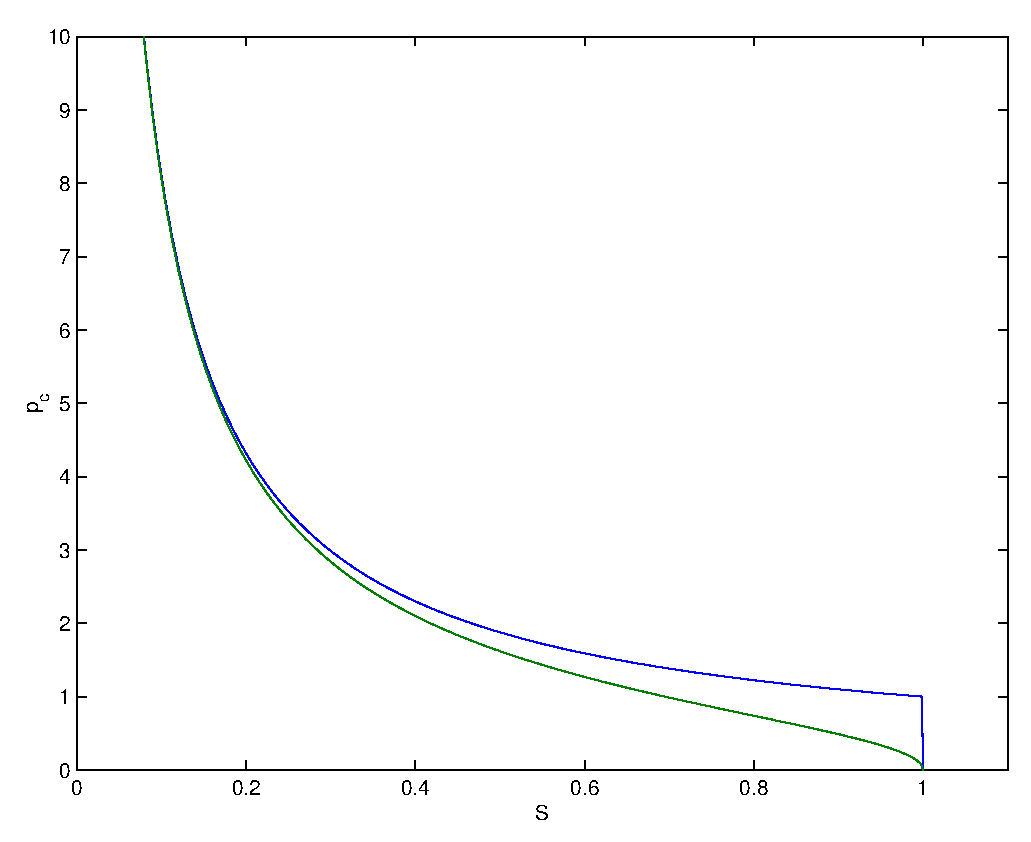
\epsfig{file=ps.eps,scale=0.5}
\end{figure}

Common $k_{r \alpha}-s_e$ relations have the shapes in figure
\ref{krplot}. The slopes can be unbounded at $s_e=1$. It turns out
that if you compose the $k_{r \alpha}-s_e$ relation with the inverse
of the $s_e(p_{ce})$ relation then the slopes of the resulting $k_{r
  \alpha}-p_{ce}$ relations are bounded for all but a small range of
cases (figure \ref{krvpcplot}). As with the $p_{ce}-s_e$ relation, the
$s_e=1$ case can be troublesome. Note that the following simplified
$k_{r \alpha}-s_e$ relations are sometimes used for analysis and
computations, but they do not exhibit all of the behavior discussed
above $s_e=1$.
\begin{eqnarray}
  \label{eq:krwSimple}
  k_{rw} &=& s_e^2 \\
  k_{rn} &=& \frac{1}{2}(1 - s_e)^2 \label{eq:krnSimple}
\end{eqnarray}

\begin{figure}
\center
\caption{$k_{r \alpha}$ vs. $s_e$ \label{krplot}}
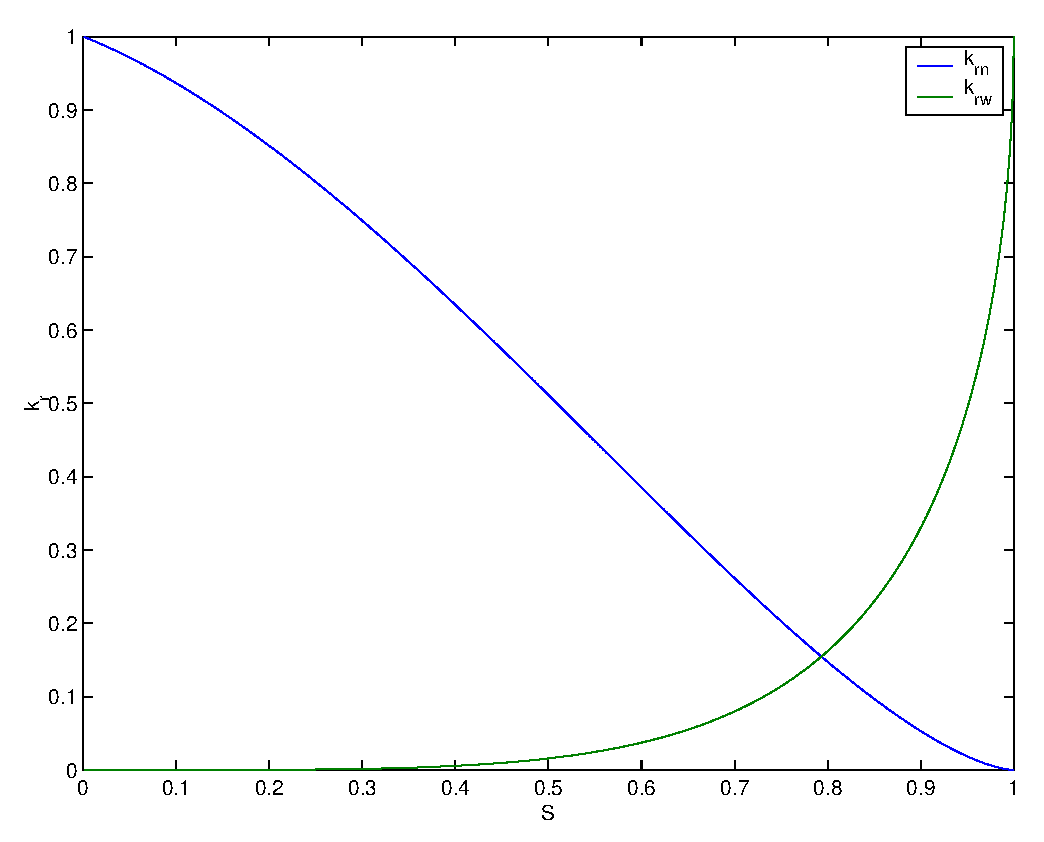
\epsfig{file=kr.eps,scale=0.5}
\end{figure}

\begin{figure}
\center
\caption{$k_{r \alpha}$ vs. $p_{ce}$ \label{krvpcplot}}
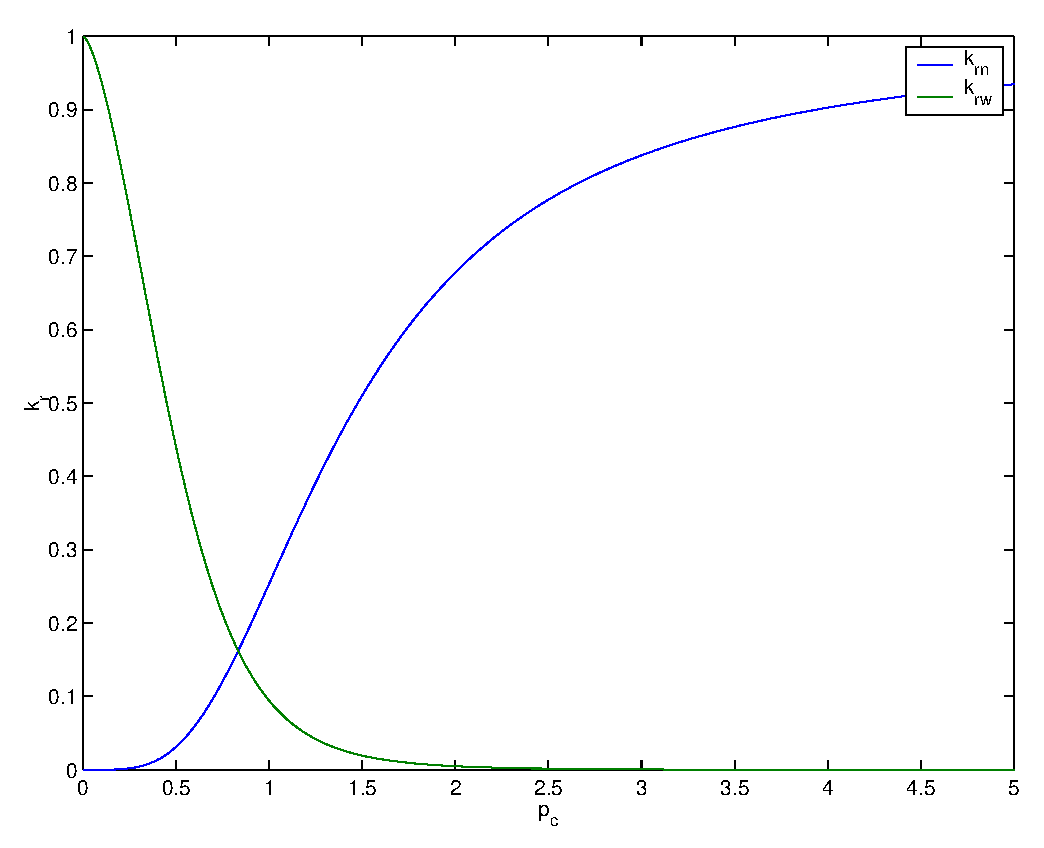
\epsfig{file=krvpc.eps,scale=0.5}
\end{figure}

The following sections work out the details of common $p-s-k$
relations for the sake of completeness. First we present $p-s$
relations. The $s-k$ relations will then be formulated independently
of the $p-s$ model. Skip to section \eqn{press_eq} if you don't need
these details, the equations and closure relations will be summarized
at the end of the chapter.

\msection{Van Genuchten} The Van Genuchten relation is
\citep{VanGenuchten_80}

\begin{eqnarray}
p_c &=& p_{ce}/\alpha\\
p_{ce} &=& \pl s_e^{-1/m} - 1 \pr^{1/n} 
\end{eqnarray}
where $n>1$, $0<m<1$, and $\alpha > 0$ ($p_{cM} = 1/\alpha$). Hence
$p_{ce}:[0,1]\rightarrow [0,\infty)$ is unbounded as $s_e
\rightarrow 0$. Furthermore
\begin{equation}
\od{p_{ce}}{s_e} = \frac{-1}{nm}\pl s_e^{-1/m} - 1 \pr^{1/n-1} s_e^{-1/m-1}
\end{equation}
is unbounded as $s_e \rightarrow 1$ and $s_e \rightarrow 0$
because $n>1$.

If we deal with the inverse instead we have
\begin{eqnarray}
s_e &=& ( 1 + p_{ce}^n)^{-m} \\
\od{s_e}{p_{ce}} &=& -mn( 1 + p_{ce}^n )^{-m-1} p_{ce}^{n-1} 
\end{eqnarray}
which is $C^1$ on $[0,\infty)$, but not $C^2$ at $p_{ce}=0$ if $1<n<2$.

\msection{Brooks-Corey} The Brooks-Corey $p - s$ relation is
\cite{Brooks_Corey_66}
\begin{eqnarray}
p_c &=& p_d p_{ce} \\
p_{ce} &=& \Big\{ \begin{array}{ll}
s_e^{-1/\lambda} & s_e < 1   \\
0 & s_e = 1 
\end{array}
\end{eqnarray}
where $\lambda > 0$ and $p_d>0$ ($p_{cM} = p_d$ is known as the
displacement or entry pressure). Thus $p_{ce}$ and $\od{p_{ce}}{s_e}$
are discontinuous at $s_e=1$ and unbounded as $s_e \rightarrow 0$. On
$(0,1)$, however, $\od{p_{ce}}{s_e}$ is bounded, as opposed to
the unbounded behavior of the van Genuchten relation.

The inverse is
\begin{equation}
s_e = \Big\{ \begin{array}{ll}
p_{ce}^{-\lambda} & p_{ce} \geq 1   \\
1 & p_{ce} < 1
\end{array}
\end{equation}
This function is $C^{\infty}$ except at $p_{ce}=1$, where it is
Lipschitz continuous.

\msection{Summary} As $s_e \rightarrow 0$, both the $p-S$ models
have $p_{ce} \rightarrow \infty$.  In fact, for small $s_e$
the curves are nearly identical if $\lambda = nm$.

At $s_e=1$ the two models differ significantly. The Brooks-Corey model
has a jump discontinuity in capillary pressure equal to the
displacement pressure (or a jump of 1 in $p_{ce}$) whereas Van
Genuchten varies continuously, but very quickly, to $p_{ce}=0$. The
non-smoothness at $s_e=1$ is significant because $s_e=1$ can be
reached with only flow processes and is often the initial condition
for a portion of the domain. We may deal with the inverses,
$s_e(p_{ce})$, in which case both curves are Lipschitz continuous on
$[0,\infty)$. The Van Genuchten curve is  $C^1$ at $p_{ce}=0$
while Brooks-Corey is Lipschitz continuous at $p_{ce}=1$. The
difference in the two curves near $S=1$ is physically significant. The
Brooks-Corey model includes the concept of finite entry pressure,
which implies that the non-wetting phase cannot jointly occupy the
pore space with the wetting phase until the non-wetting phase pressure
exceeds $p_d$.  Recent work suggests that the Van Genuchten curves
should be augmented with a finite entry pressure
\citep{Gerhard_Kueper_03a,Gerhard_Kueper_03b}.

\msection{Permeability Models} The permeability models are based on
empirical and theoretical considerations that relate the saturation
and the capillary pressure to the permeability. For that reason they
depend on the $p-S$ relations above. We first present the general
permeability models and then derive closed form expressions for the
permeability functions using the Brooks-Corey and Van Genuchten $p-s$
relations.

\msection{Mualem} Mualem's general permeability model is
\citep{Mualem_76}
\begin{eqnarray}
k_{rw} &=& s_e^{1/2} \cbl \frac{\int_0^{s_e} \frac{1}{p_c} ds }{\int_0^1 \frac{1}{p_c} ds } \cbr^2\\
k_{rn} &=& (1 - s_e)^{1/2} \cbl \frac{\int_{s_e}^1 \frac{1}{p_c} ds }{ \int_0^1 \frac{1}{p_c} ds}  \cbr^2
\end{eqnarray}

\msection{Burdine} Burdine's general permeability model is
\citep{Burdine_53}
\begin{eqnarray}
k_{rw} &=& s_e^2 \cbl \frac{\int_0^{s_e} \frac{1}{p_c^2} ds }{\int_0^1 \frac{1}{p_c^2} ds } \cbr\\
k_{rn} &=& (1 - s_e)^2 \cbl \frac{\int_{s_e}^1 \frac{1}{p_c^2} ds }{ \int_0^1 \frac{1}{p_c^2} ds}  \cbr
\end{eqnarray}

\msection{Van Genuchten-Mualem} Note that both models above are
independent of scalings of $p_c$, so that we simply use $p_{ce}$
for the calculations. If we substitute the Van Genuchten $p-s$ model
into the Mualem permeability model we need to calculate the integral
\begin{equation}
\int_0^{s_e}  \pl s_e^{-1/m} - 1 \pr^{-1/n}ds
\end{equation}
Making the substitution $y^m=s_e$ and requiring that $m=1 - 1/n$
we obtain \citep{VanGenuchten_80}
\begin{eqnarray}
m \int_0^{y^m}  \pl y^{-1} - 1 \pr^{-1/n} y^{m-1} dy &=& m \int_0^{y^m}  \pl \frac{1-y}{y}\pr^{-1/n} y^{m-1} dy \\
&=& m \int_0^{y^m}  \pl 1-y \pr^{-1/n} y^{m-1+1/n} dy \\
&=& m \int_0^{y^m}  \pl 1-y \pr^{-1/n}  dy \\
&=& -\frac{m}{1-1/n}(1-y)^{1-1/n} |_0^{y^m} \\
&=& 1 - (1 - s_e^{1/m})^m
\end{eqnarray}
Hence
\begin{eqnarray}
k_{rw} &=& s_e^{1/2} \sbl 1-(1-s_e^{1/m})^m \sbr^2 \\
k_{rn} &=& (1-s_e)^{1/2}(1-s_e^{1/m})^{2m}
\end{eqnarray}
and
\begin{eqnarray}
\od{k_{rw}}{s_e} &=& \frac{1}{2}s_e^{-1/2}\sbl 1 - \pl 1 - s_e^{1/m}\pr^m \sbr^2 \\
&&+2 \sbl 1- \pl 1- s_e^{1/m}\pr^m \sbr \pl 1-s_e^{1/m} \pr^{m-1} s_e^{1/m-1/2} \\
\od{k_{rn}}{s_e} &=& -\frac{1}{2}(1-s_e)^{-1/2} (1-s_e^{1/m})^{2m} \\
&&-2(1-s_e)^{1/2}(1-s_e^{1/m})^{2m-1} s_e^{1/m-1}
\end{eqnarray}

Since $0 < m< 1$, $\od{k_{rw}}{s_e}$ and $\od{k_{rn}}{s_e}$
may be unbounded as $s_e \rightarrow 1$.

Substituting the Van Genuchten $s-p$ relationship we obtain
\begin{eqnarray}
k_{rw} &=& \frac{ \sbl 1 - p_{ce}^{n-1} \pl1 + p_{ce}^n \pr^{-m} \sbr^2}{\pl 1 + p_{ce}^n \pr^{m/2} } \\
k_{rn} &=& \sbl 1 - \pl1  + p_{ce}^n \pr^{-m} \sbr^{1/2}  \sbl p_{ce}^{n-1} \pl1 + p_{ce}^n \pr^{-m} \sbr^2
\end{eqnarray}
and
\begin{eqnarray}
k_{rw} &=& \frac{-nm}{2}\pl 1 + p_{ce}^n \pr^{-m/2-1} p_{ce}^{n-1}  \sbl 1 - p_{ce}^{n-1} \pl1 + p_{ce}^n \pr^{-m} \sbr^2 +\\
&& -2\pl 1 + p_{ce}^n \pr^{-m/2}  \sbl 1 - p_{ce}^{n-1} \pl1 + p_{ce}^n \pr^{-m} \sbr \cdot \\
&&\sbl (n-1)p_{ce}^{n-2} \pl1 + p_{ce}^n \pr^{-m} -mn p_{ce}^{n-1} \pl1 + p_{ce}^n \pr^{-m-1}p_{ce}^{n-1}\sbr\\
k_{rn} &=& \frac{-nm}{2}\sbl 1 - \pl1  + p_{ce}^n \pr^{-m} \sbr^{-1/2} \pl1  + p_{ce}^n \pr^{-m-1} p_{ce}^{n-1}\sbl p_{ce}^{n-1} \pl1 + p_{ce}^n \pr^{-m} \sbr^2 \\
&&2\sbl 1 - \pl1  + p_{ce}^n \pr^{-m} \sbr^{1/2}  \sbl p_{ce}^{n-1} \pl1 + p_{ce}^n \pr^{-m} \sbr \cdot \\
&&\sbl (n-1)p_{ce}^{n-2} \pl1 + p_{ce}^n \pr^{-m} -nm p_{ce}^{n-1} \pl1 + p_{ce}^n \pr^{-m-1} p_{ce}^{n-1}\sbr
\end{eqnarray}
Using this form of the relations we only get unbounded derivatives in
$k_{rw}$ at $p_c=0$ in the case $1<n<2$, which is the same range where
the second derivative of the Van Genuchten $p-S$ relation is unbounded
at $p_c=0$.
 
\msection{Van Genuchten-Burdine} Similar manipulations to the Mualem
model requiring that $m=1 - 2/n$ lead to
\begin{eqnarray}
k_{rw} &=& s_e^2 \sbl 1 - \pl1 - s_e^{1/m} \pr^m \sbr \\
k_{rn} &=& \pl 1-s_e \pr^2 \pl 1-S^{1/m} \pr^{m}
\end{eqnarray}
or
\begin{eqnarray}
k_{rw} &=& \frac{1 - p_{ce}^{n-1} \pl1 + p_{ce}^n \pr^{-m}}{\pl 1 + p_{ce}^n \pr^{2m} } \\
k_{rn} &=& \sbl 1 - \pl1  + p_{ce}^n \pr^{-m} \sbr^{2}  \sbl p_{ce}^{n-1} \pl1 + p_{ce}^n \pr^{-m} \sbr
\end{eqnarray}

\msection{Brooks-Corey-Mualem} Again substituting the $p_c - S$
relation into the Mualem expression we obtain
\begin{eqnarray}
k_{rw} &=& s_e^{(4+5\lambda)/ 2 \lambda}\\
k_{rn} &=& (1-s_e)^{1/2} (1 - s_e^{1/\lambda + 1})^2
\end{eqnarray}
or
\begin{eqnarray}
k_{rw} &=& p_{ce}^{-(4+5\lambda)}\\
k_{rn} &=& (1-p_{ce}^{-\lambda})^{1/2} (1 - p_{ce}^{-(\lambda +1)})^2
\end{eqnarray}

\msection{Brooks-Corey-Burdine} Using the Burdine model (which is
typically used in conjunction with Brooks-Corey) gives
\begin{eqnarray}
k_{rw} &=& s_e^{(2 + 3 \lambda)/\lambda} \\
k_{rn} &=& (1-s_e)^2(1-s_e^{(2+\lambda)/\lambda}) 
\end{eqnarray}
or
\begin{eqnarray}
k_{rw} &=& p_{ce}^{-(2 + 3 \lambda)} \\
k_{rn} &=& (1-p_{ce}^{-\lambda})^2(1-p_{ce}^{-(2+\lambda)}) 
\end{eqnarray}

\subsection{Working Formulations}

\subsubsection{Dimensionless Variables}
\begin{eqnarray}
\tilde{t} &=& t \sqrt{\frac{g}{l}} \\
\tilde{\vec x} &=& \vec x \frac{1}{l} \\
\tilde{\psi}_{\alpha} &=& \frac{p_{\alpha} - p_{w,0}}{\rho_{w,0} g l} \label{eq:head2p}\\
\tilde{\psi}_c &=& \tilde{\psi}_n - \tilde{\psi}_w \label{eq:capHead}\\
\tilde{\rho}_{\alpha} &=& \frac{\rho_{\alpha}}{\rho_{\alpha,0}} \\
\tilde{\ten K} &=& \frac{\rho_{w,0} g \ten k}{\mu_w \sqrt{gl}} \\
\tilde{\vec v}_{\alpha} &=& \vec v_{\alpha} \frac{1}{\sqrt{gl}} \\
\tilde{\vec g} &=& \frac{\vec g}{g} \label{eq:dg2p} \\
\tilde{z} &=& -\tilde{\vec g} \cdot (\tilde{\vec x} - \tilde{\vec x}_0) \\
\tilde{\mu_{\alpha}} &=& \frac{\mu_{\alpha}}{\mu_w}\\
\tilde{\lambda}_w &=& \frac{\tilde{\rho}_w k_{rw}}{\tilde{\mu}_w}\\
\tilde{\lambda}_n &=& \frac{\tilde{\rho}_n k_{rn}}{\tilde{\mu}_n}\\
\tilde{c}_{\alpha} &=& \frac{c_{\alpha}}{\rho_{\alpha,0}}\sqrt{\frac{l}{g}} \\ 
\tilde{d}_{\alpha} &=& \frac{d_{\alpha}}{\rho_{\alpha,0}}\sqrt{\frac{l}{g}} \\
b &=& \frac{\rho_{n,0}}{\rho_{w,0}}
\end{eqnarray}

\subsubsection{Pressure-Saturation Equations \label{eq:press_eq}}

Substituting \eqns{waterFlux}{viscosity} into \eqnst{satW}{satN} and
writing the result in terms of the dimensionless variables above
(dropping the tilde's) yields:
\begin{eqnarray}
\pd{\omega s_w \rho_w}{t} + \deld \pl \rho_w \vec v_w \pr + c_w&=& d_w \label{eq:satPrim} \\
\rho_w \vec v_w &=& -\ten{K} \lambda_w \pl \grad \psi_w + \rho_w \grad z \pr  \\
\pd{\omega (1-s_w) \rho_n}{t} + \deld \pl \rho_n \vec v_n \pr + c_n&=& d_n \\
\rho_n \vec v_n &=& -\ten{K} \lambda_n \pl \grad \psi_w + \grad \psi_c + b \rho_n \grad z \pr \label{eq:qnPrim}
\end{eqnarray}
The choice of the two unknowns depends on how general we wish the
model to be. Since incompressible fluids and media are often used in
practice $\omega$ and $\rho_\alpha$ are ruled out. On the other hand
the phase pressures cannot be determined as functions of $S_n$, $S_w$,
and $p_c$, so at least one phase pressure is usually included as a
dependent variable.  Lastly, in the case of the disappearance of one
of the phases under incompressibility assumptions, the Darcy's law for
that phase has zero coefficients in the spatial terms so only the
temporal accumulation term remains, leaving only the temporal term for
the saturation. If $\od{S}{p_c}=0$ under these conditions (i.e. the
Van Genuchten $p-S$ relation), applying the chain rule will still not
produce an equation for $p_c$. For these reasons the most versatile
choice appears to be a phase pressure and a saturation, say
$(S_w,p_w)$. This formulation is called the pressure-saturation
formulation (c.f.  \citep{Aziz_Settari_79,Chavent_Jaffre_86,
  Helmig_97}). Further discussion of the choice of variables can be
found in \citep{Kueper_Frind_91,Kees_Miller_02}. Since the
constitutive theory is based on wetting phase fluid being present at
every point in the medium, $S_w$ and $p_w$ always have physical
meaning.

\subsubsection{Fractional Flow Formulations}

The petroleum industry generally uses formulations based on the total
fluid velocity, that is, the sum of both phase velocities. The wetting
phase mass balance is then rewritten in terms of this total velocity
by formulating the so-called ``fractional flow'' function. We explore
several formulations based on this approach (c.f.
\citep{Chavent_Jaffre_86}).

Summing \eqns{satPrim}{qnPrim} we obtain
\begin{eqnarray}
  \label{eq:totalmb}
  \pd{\omega \sbl \rho_w s_w + \rho_n (1-s_w)\sbr}{t} + \deld \pl \rho_w \vec v_v + \rho_n \vec v_n \pr &=& 0 \\
\rho_w \vec v_v + \rho_n \vec v_n &=& -\ten{K} \sbl \pl \lambda_w + \lambda_n \pr \grad \psi_w + \lambda_n \grad \psi_c \right. \\
&& \left. + \pl \lambda_w \rho_w  + \lambda_n b \rho_n \pr \grad z \sbr  
\end{eqnarray}
To simplify further we define
\begin{eqnarray}
  \vec q_t &=& \rho_w \vec v_v + \rho_n \vec v_n \\
  \lambda_t &=&  \lambda_w + \lambda_n \\
  f_n &=& \frac{\lambda_n}{\lambda_t}\\
  f_w &=& \frac{\lambda_w}{\lambda_t} \\
  \rho_t &=& f_w\rho_w  + f_n b \rho_n = \rho_w + f_n (b \rho_n - \rho_w)
\end{eqnarray}
Note that $f_n + f_w = 1$. Substituting these definitions yields
\begin{eqnarray}
  \label{eq:totalHet}
  \pd{\omega \sbl s_w \pl \rho_w - \rho_n \pr + \rho_n \sbr }{t} + \deld \vec q_t &=& 0 \\
\vec q_t &=& - \ten{K} \lambda_t \pl \grad \psi_w + f_n \grad \psi_c + \rho_t \grad z \pr
\end{eqnarray}
Now we express $\rho_w \vec v_w$ in terms of $\vec q_t$. Note first that 
\begin{equation}
  \label{eq:fracflow}
  f_w \vec q_t = -\ten{K} \cbl \lambda_w \grad \psi_w + \lambda_w f_n \grad \psi_c + \lambda_w \sbl \rho_w + f_n \pl b \rho_n - \rho_w \pr \sbr  \grad z \cbr
\end{equation}
Hence, we obtain for $\rho_w \vec v_w$
\begin{equation}
\rho_w \vec v_w = f_w \vec q_t + \ten{K} \lambda_w \ten f_n \grad \psi_c + \ten{K} \lambda_w f_n \pl  b \rho_n -\rho_w\pr \grad z 
\end{equation}
Combining the results yields
\begin{eqnarray}
\pd{\omega \rho_w s_w}{t} + \deld \vec q_w &=& 0 \\
\vec q_w &=&  f_w \vec q_t + \ten{K} \lambda_w f_n \grad \psi_c + \ten{K} \lambda_w f_n \pl  b \rho_n -\rho_w \pr \grad z \\
\pd{\omega \sbl s_w \pl \rho_w - \rho_n \pr + \rho_n \sbr }{t}+ \deld \vec q_t &=& 0 \\
\vec q_t  &=& - \ten{K} \lambda_t \pl \grad \psi_w + f_n \grad \psi_c + \rho_t \grad z \pr 
\end{eqnarray}
If we choose $s_w, \psi_w$ as the dependent variables and assume
$\psi_c = \psi_{cM}(\vec x) \bar{\psi}_c(S_w)$ then using the chain
rule on $\grad \psi_c$ yields
\begin{eqnarray}
\pd{\omega \rho_w S_w}{t} + \deld (\vec q_w) &=& 0 \\
\vec q_w &=&  f_w \vec q_t + \ten{K} \lambda_w f_n \pl \psi_{cM} \od{\bar{\psi}_c}{S_w} \grad S_w + \bar{\psi_c} \grad \psi_{cM} \pr \\
&& + \ten{K} \lambda_w f_n \pl  b \rho_n -\rho_w \pr \grad z \\
\pd{\omega \sbl S_w \pl \rho_w - \rho_n \pr + \rho_n \sbr }{t} + \deld \vec q_t &=& 0 \\
\vec q_t  &=& - \ten{K} \lambda_t \pl \grad \psi_w + f_n \od{\psi_c}{S_w} \grad S_w + \rho_t \grad z \pr 
\end{eqnarray}

\subsubsection{Potentials}

Defining potentials to remove nonlinear diffusion terms can be more
complicated in the two-phase case because nonlinearities may have more
complicated dependencies. In general we may have a term like
$a(u,v,\vec x) \grad u$ that we would like to write as $\grad \phi$
for some $\phi$. Using the Kirchoff transform we get for $i=1,2,3$
\begin{equation}
  \label{eq:kirchmp}
  \pd{\int_{u_0}^{u} a(w,v,\vec x) dw}{x_i} = a(u,v,w) u_{x_{i}} + \int_{u_0}^{u} \pd{a}{v}(w,v,\vec x) dw \pd{v}{x_i} + \int_{u_0}^{u} \pd{a}{x_i}(w,v,\vec x) dw
\end{equation}
so in general to employ a potential we have to incorporate
``correction'' terms (the last two terms on the rhs)
\begin{equation}
  \label{eq:kirchgen}
  a(u,v,\vec x) \grad u = \grad \phi - \chi \grad v - \grad A
\end{equation}
where
\begin{eqnarray}
  \label{eq:kirchdeff}
  \phi &=& \int_{u_0}^{u} a(w,v,\vec x) dw \\
  \chi  &=& \int_{u_0}^{u} \pd{a}{v}(w,v,\vec x) dw \\
  \pl \grad A \pr_i &=&  \int_{u_0}^{u} \pd{a}{x_i}(w,v,\vec x) dw \quad i=1,2,3
\end{eqnarray}

\subsubsection{Global Pressure Formulation}

In the total flow equation if we use the approach in the previous
section to define a potential
\begin{equation}
  \label{eq:cap}
\phi = \int_{-\infty}^{\psi_c} f_n(w) dw 
\end{equation}
then
\begin{eqnarray}
\vec q_t  &=& - \ten{K} \lambda_t \pl \grad \psi_w + \grad \phi - \chi \grad \psi_w - \grad A + \rho_t \grad z \pr 
\end{eqnarray}
This form motivates the definition of a global pressure head
\begin{equation}
  \label{eq:globalHead}
  \psi_t = \psi_w + \phi = \psi_w + \int_{-\infty}^{\psi_c} f_n(w) dw
\end{equation}
The global pressure can also be rewritten in a more intuitive form using the facts that $f_n = 1 - f_w$ and $\psi_c = \psi_n - \psi_w$:
\begin{equation}
  \label{eq:globalHeadAvg}
  \psi_t = \frac{\psi_w + \psi_n}{2} + \phi^* = \frac{\psi_w + \psi_n}{2} + \int_{-\infty}^{\psi_c} \sbl \frac{1}{2} - f_w(w) \sbr dw
\end{equation}
If we assume that the densities involved in $\phi$ (through $f_n$) are
evaluated at $\psi_t$ rather than $\psi_w$, we can make
\eqn{globalHead} or \eqn{globalHeadAvg} an implicit definition of
$\psi_t$, and we obtain for the global flow
\begin{eqnarray}
\vec q_t  &=& - \ten{K} \lambda_t \pl (1 - \chi) \grad \psi_t - \grad A + \rho_t \grad z \pr 
\end{eqnarray}
The global pressure gathers all the pressure effects into a single
potential, which from \eqn{globalHeadAvg} we see is an extention of
the arithmetic average of the phase pressures, which incorporates
capillary effects.

\subsubsection{Homogeneous Relative Permeabilities}

If we can write the relative permeabilities as
\begin{equation}
  \label{eq:factoredRelPerm}
  k_{r\alpha} =k_r(\vec x) k_{r\alpha}(s_e)
\end{equation}
then the spatial dependence is essentially part of the hydraulic
conductivity anyway, so we can assume it is incorporated into
$\bar{K}$ and the term $\grad A$ is then zero.

\subsubsection{Incompressible Fluids} 

If, additionally, the fluids are incompressible then $\rho_n = \rho_w
= 1$ (recall that we're using dimensionless variables) and the cross term $\chi$
above is zero, which yields
\begin{eqnarray}
\deld \vec q_t &=& 0 \\
\vec q_t  &=& - \ten{K} \lambda_t \pl \grad \psi_t + \rho_t \grad z \pr 
\end{eqnarray}
In one dimension this reduces to $\vec q(\vec x,t) = \vec q(t)$ and
the system effectively reduced to a single nonlinear equation for the
$s_w$.

\subsubsection{Light, Inviscid Non-Wetting Phase}

If we assume $\mu_n / \mu_w = 0$ then $f_n = 1$ and $f_w =0$ except
possibly in the limits as $s_w \rightarrow 0,1$ so that the saturation
equation reduces to
\begin{eqnarray}
\pd{\omega \rho_w s_w}{t} + \deld  \vec q_w  &=& 0 \\
\vec q_w &=& \ten{K} \lambda_w \grad \psi_c + \ten{K} \lambda_w \pl  b \rho_n - \rho_w \pr \grad z 
\end{eqnarray}
Furthermore if we assume $b = \rho_{n,0}/\rho_{w,0} = 0$ then no terms
depend on the properties of the non-wetting fluid.

\subsubsection{Richards' Equation}

If we fix $\psi_n = 0$ then $\psi_c = - \psi_w$ and we obtain
Richards' equation
\begin{eqnarray}
  \pd{\omega \rho_w s_w}{t} + \deld \vec q_w &=& 0 \\
  \vec q_w &=& -\ten{K} \lambda_w \pl \grad \psi_w + \rho_w \grad z
  )\pr
\end{eqnarray}

\subsection{Boundary and Initial Conditions}

Boundary conditions can get very complicated in two-phase flow because
of the wide range of variable choices. As mentioned above the most
versatile model of two-phase flow outside of the fractional flow model
uses $s_w$ and $\psi_w$. This choice can also be used in the
fractional flow model. On the other hand if $\psi_t$ is used instead,
then of course simple linear Dirichlet conditions on $\psi_w,s_w$
become nonlinear Dirichlet conditions on $\psi_t,s_w$.

\begin{center}
\fbox{\begin{minipage}[b]{6.5in}
\subsection{Summary}
Two-Phase Flow Equations
\begin{eqnarray}
m_{1,t} + \deld \pl \vec f_1 - \sum_{j=1}^2 \ten{a}_{1,j} \grad \phi_j \pr + c_1 = d_1 \\
m_{2,t} + \deld \pl \vec f_2 - \sum_{j=1}^2 \ten{a}_{2,j} \grad \phi_j \pr + c_2 = d_2 
\end{eqnarray}
\begin{align}
c_{\alpha},d_{\alpha} &= \mbox{problem dependent wells and sources} \\
\intertext{Auxiliary Variables (Dimensionless) }
\lambda_w &= \frac{\rho_w k_{rw}}{\mu_w}\\
\lambda_n &= \frac{\rho_n k_{rn}}{\mu_n}\\
\lambda_t &=  \lambda_w + \lambda_n \\
f_n &= \frac{\lambda_n}{\lambda_t}\\
f_w &= \frac{\lambda_w}{\lambda_t}\\
\rho_t &= f_w\rho_w  + f_n b \rho_n = \rho_w + f_n (b \rho_n - \rho_w)\\
\end{align}
\end{minipage}}
\end{center}

\begin{center}
\fbox{\begin{minipage}[b]{6.5in}
\begin{align}
\intertext{Primitive Form Coefficients}
m_{1} &= \omega \rho_w s_w \\
m_{2} &= \omega \rho_n (1-s_w) \\
f_1 &= - \rho^{2}_{w} \ten{K} \lambda_w \grad z \\
f_2 &= - \rho^{2}_{n} \ten{K} \lambda_n b \grad z \\
\ten{a}_{1,1} &= \rho_w \ten{K} \lambda_w\\
\ten{a}_{2,2} &= \rho_n \ten{K} \lambda_n\\
\phi_{1} &= \psi_w \\
\phi_{2} &= \psi_c(s_w) + \psi_w\\
u_1 &= s_w \\
u_2 &= \psi_w 
\intertext{Fractional Flow (``Phase Form'') Coefficients}
m_{1} &= \omega \rho_w s_w\\
m_{2} &= \omega \sbl s_w (\rho_w - \rho_n) + \rho_n \sbr\\
f_{1} &= f_w q_t + \ten{K} \lambda_w f_n (b \rho_n - \rho_w) \grad z \\
f_{2} &= \ten{K} \lambda_t \rho_t \grad z\\
a_{1,1} &= -\ten{K} \lambda_w f_n\\
a_{2,1} &= \ten{K} \lambda_n \\
a_{2,2} &= \ten{K} \lambda_t \\
\phi_1 &= \psi_c(s_w) \\
\phi_2 &= \psi_w \\ 
u_1 &= s_w \\
u_2 &= \psi_w\\
  \intertext{Fractional Flow (``Global Pressure'')}
  m_{1} &= \omega \rho_w s_w\\
  m_{2} &= \omega \sbl s_w (\rho_w - \rho_n) + \rho_n \sbr\\
  f_{1} &= f_w q_t + \ten{K} \lambda_w f_n (b \rho_n - \rho_w) \grad z \\
  f_{2} &= \ten{K} \lambda_t \rho_t \grad z\\
  a_{1,1} &= -\ten{K} \lambda_w f_n\\
  a_{2,2} &=  \ten{K} \lambda_t (1-\chi) \\
  \phi_1 &= \psi_c(s_w) \\
  \phi_2 &= \psi_t = \psi_w + \int_{-\infty}^{\psi_c}  f_n(w) dw = \frac{\psi_w + \psi_n}{2} + \int_{0}^{s_e} \pl \frac{1}{2} - f_w \pr \od{\psi_c}{s_e} dw\\
  u_1 &= s_w \\
  u_2 &= \psi_t \\
\intertext{Richards' Equation}
m_1 &= \omega \rho_w s_w\\
f_1 &= -\ten{K} \lambda_w \rho_w \grad z \\
a_1 &= \ten{K} \lambda_w \\
\phi_1 &= \psi_w \\
u_1 &= \psi_w
\end{align}
\end{minipage}}
\end{center}
\begin{center}
\fbox{\begin{minipage}[b]{6.5in}
\begin{align}
  \intertext{p-s-k Closure Relations}
  s_e &= \frac{s_w -  s_m(\vec x)}{s_M(\vec x) - s_m(\vec x)} && \mbox{(effective saturation)}\\
  p_{ce} &= \frac{p_c}{p_{cM}(\vec x)} && \mbox{(effective capillary pressure)}\\
  \intertext{\center Simple Model}
  p_{ce} &= s_e \\
  k_{rw} &= s_e^2  \\
  k_{rn} &= \frac{1}{
2}(1-s_e)^2
  \intertext{\center Van Genuchten-Mualem}
  p_{cM} &= \frac{1}{\alpha(\vec x)} && \alpha > 0\\
  p_{ce} &= \pl s_e^{-1/m} - 1 \pr^{1-m} && 0 < m < 1\\
  k_{rw} &= s_e^{1/2} \sbl 1-(1-s_e^{1/m})^m \sbr^2 \\
  k_{rn} &= (1-s_e)^{1/2}(1-s_e^{1/m})^{2m} \\
  \intertext{\center Brooks-Corey-Burdine}
  p_{cM} &= p_d(\vec x) &&p_d > 0\\
  p_{ce} &= \Big\{ \begin{array}{ll}
    s_e^{-1/\lambda} & s_e < 1   \\
    0 & s_e = 1 
  \end{array} && \lambda > 0\\
  k_{rw} &= s_e^{(2 + 3 \lambda)/\lambda} \\
  k_{rn} &= (1-s_e)^2(1-s_e^{(2+\lambda)/\lambda}) 
\end{align}
Notes: i) In any of the above formulations a nonlinear potential, such
as $\psi_c(s_w)$ can be chained out to get a diffusion term with
respect to the unknown ($s_w$). It's probably better to avoid doing
that because 1) it makes the Jacobian of the fully discrete model more
complicated 2) it relies on more smoothness in $\psi_c(s_w)$, and 3) I
have a vague idea that you want to avoid putting nonlinearity in the
diffusion coefficients (the a's). ii) The density and porosity closure
relations are the same as for the saturated case. 
\end{minipage}}
\end{center}

% \section{Analysis}

% \subsection{Overview}

% Our goal is solving systems of nonlinear advection-diffusion-reaction
% equations of the form
% \begin{equation}
%   \label{eq:nladrsys}
%   \pd{m^i}{t} + \deld \sbl \vec f^i - \sum_{j=1}^{n_c} \ten{a}^{ij} \grad \phi^j \sbr + c^i = d^i \mbox{ in } (0,T] \times U \mbox{ for } i=1,\ldots, n_c
% \end{equation}
% where $n_c$ is the number of components and $U$ is a usually bounded
% open subset of $\R^3$. The coefficients $m^i$, $\vec f^i$,
% $\ten{a}^i$, $\phi^i$, and $c^i$ are considered to be functions of $t,
% \vec x, u^1, \ldots, u^{n_c}$ where $u^i: (0,T] \times U =U_T
% \rightarrow \R$ are the components of the solution. The source term
% $d^i$ is a function of $t$ and $\vec x$ only. The boundary conditions
% may be written as
% \begin{equation}
%   \label{eq:bc}
%   G^i(x,t,u^1,\dots,u^{n_c}) = 0 \mbox{ on } (0,T] \times \partial U 
% \end{equation}
% and usually take the form
% \begin{eqnarray}
% \sbl \vec f^i - \sum_{j=1}^{n_c} \ten{a}^{ij} \grad \phi^j \sbr \cdot \gvec \nu  &=& g^i_N(x,t,u^1,\dots,u^{n_c}) \mbox{ on } (0,T] \times \partial U_N \\
% u^i  &=& g^i_D(x,t,u^1,\dots,u^{n_c}) \mbox{ on } (0,T] \times \partial U_D
% \end{eqnarray}
% Note that since we leave open whether $g^i_N$ can be solution-dependent we can express mixed (Robin) boundary conditions via $g^i_N$, i.e.
% \begin{equation}
% \sbl \vec f^i - \sum_{j=1}^{n_c} \ten{a}^{ij} \grad \phi^j \sbr \cdot \gvec \nu  = \frac{\alpha (u - g^i_D) + \beta \hat{f}_N}{\beta}
% \end{equation}
% The initial conditions are
% \begin{equation}
%   \label{eq:ic}
%   u^i(x,0) = u^i_0(x) \mbox{ on } \bar{U}
% \end{equation}
% We are interested in solutions $u$, which lie in some space of
% functions $X$ defined on $U_T$. If we can show that a solution exists
% then we have effectively shown that there is a mapping, $S$, on the
% data of the problem (e.g. $u_0,d$,...) such that $u =
% S(u_0,d,p_1,\ldots,p_m)$ satisfies the equation in some sense that is
% relevant for functions in $X$. Since we focus on physical problems
% where the data cannot be known with infinite precision, the solution
% operator is also required to be continuous with respect to the data.
% For example, if we consider continuity with respect to the initial
% data $u_0 \in X$ where $X$ is endowed with a norm $\|.\|_X$, then we
% would like to know that there exists a $\delta > 0$ such that for
% every $\epsilon > 0$
% \begin{equation}
%   \label{eq:contDep}
%   \|S(v_0) - S(u_0)\|_X  < \epsilon \mbox{ if } \| v_0 - u_0 \|_X < \delta 
% \end{equation}
% This continuity with respect to the data has many other formulations:
% for linear operators boundedness and continuity are equivalent so the
% focus of analysis is on proving that the inverse is bounded. More
% generally if $X$ is considered with respect to a topology
% $\mathcal{T}$ and the space $(X,mathcal{T})$ is not endowed with a
% norm then we might consider the basic topological definition of
% continuity: for all open $V \subset X$, $S^{-1}(V)$ is open.
% Additionally, we usually want to know whether the solution is unique
% and whether perhaps it lies in some smaller space than $X$, the latter
% question usually being a question of the regularity of solutions on
% $U_T$. For example we may have found a solution in $L_2(U)$ but are
% able to identify these solutions with $C^{\infty}(U)$ functions. For concreteness recall the finite dimensional linear and nonlinear problems:
% \begin{equation}
%   \label{eq:linearFinite}
%   A x = b \mbox{for} A \in \R^{n\times n}, x,b \in \R^{n}
% \end{equation}
% We know that if the $\det(A) \neq 0$ then there is a unique solution
% for all $b \in \R^n$.  We denote this solution $A^{-1}(b)$. Since $A$
% is linear $A (\alpha A^{-1}(b) + A^{-1} (c)) = \alpha b + c =
% A^{-1}(\alpha b + c)$. By the uniqueness of $A^{-1}(\alpha b + c)$, we
% have that $A^{-1}$ is linear. In $\R^n$ all linear operators are
% bounded so 

% For a classical solution, if the coefficients are
% sufficiently regular, say $C^{\infty}(U_T \times \R^{n_c})$, then we
% could define
% \begin{equation}
% X = C^2_1(U_T) = \cbl u^i: U_T \rightarrow \R | u^i, \pd{u^i}{t}, \pd{u^i}{x_j}, \pdsm{u^i}{x_j}{x_k}  \in C(U_T), j,k=1,2,3 \cbr  
% \end{equation}
% If the coefficients and boundary conditions are independent of time,
% we can also think of the equation as an autonomous ordinary
% differential equation on $X=C^2(U)$
% \begin{equation}
%   \label{eq:classicalEvolution}
%   \od{u^i}{t} = F^i(u^1,\ldots,u^{n_c}) \quad i = 1,\ldots,n_c 
% \end{equation}
% where $F^i: X^{n_c} \rightarrow \R$ and $u^i \in C^1((0,T],X)$. The
% norm on $X$ could be
% \begin{equation}
% \|u^i(t)\|_{X} = \sup_{x \in U} |u^i(t,x)|
% \end{equation}
% and the time derivative above is the linear map $\od{u^i}{t}(t):\R \rightarrow X$ satisfying
% \begin{equation}
%   \label{eq:frechet}
%  \lim_{\epsilon\rightarrow 0} \|\frac{u^i(t + \epsilon s) - u^i(t)}{\epsilon} - \od{u^i}{t}(t) s \|_{X} = 0 
% \end{equation}
% The coefficients and solutions are often not smooth enough to justify
% the interpretations of the equations above; therefore, instead of
% seeking classical solutions, various weak formulations of
% \eqns{nladrsys}{ic} are used.

% As a first step away from a classical (pointwise) interpretation of
% the problem, consider the case when the coefficients are smooth and
% independent of time and the boundary conditions are $u|_{\partial U} =
% 0$. The right hand side of \eqn{classicalEvolution} is in $L^2(U)$ as
% long as $u$ is in the Sobolev space $W^{2,2}(U)=H^2(U)$, that is the spatial
% derivatives have $L^2(U)$ representations. Furthermore $u$ satisfies
% the boundary conditions as long as $u \in H^1_0(U) \cap
% H^2(U)$ where $H^1_0(U)$ is the closure of $C^{\infty}_c(U)$
% in $H^1(U)$ or equivalently $u|_{\partial U} = 0$ in the trace
% sense. We can now interpret \eqn{classicalEvolution} as an evolution
% equation on $L^2(U)$ where the domain of $F^i$ is $H^1_0(U) \cap
% H^2(U)$. The time derivative $\od{m}{t}$ is then interpreted in
% the sense of $L^2(U)$. This is the semigroup view of the equation.

% Next consider the steady state equation
% \begin{equation}
%   \label{eq:steadyState}
%   \deld \sbl \vec f^i - \sum_{j=1}^{n_c} \ten{a}^{ij} \grad \phi^j \sbr + c^i = s^i \mbox{ in } U 
% \end{equation}
% with boundary conditions $u^i|_{\partial U} = 0$.  Multiplying
% \eqn{steadyState} by a test function $w^i \in C^{\infty}_c(U)
% \rightarrow \R$ (that is, the support of $w$ is a compact set
% contained in $U$) and integrating by parts yields
% \begin{eqnarray}
%   \label{eq:weakSteadyState}
%   -\int_{U} \cbl \sbl \vec f^i - \sum_{j=1}^{n_c} \ten{a}^{ij} \grad \phi^j \sbr \cdot \grad w^i + c^iw^i \cbr dU &=& \int_{U} s^iw^i dU - \int_{\partial U} \sbl \vec f^i - \sum_{j=1}^{n_c} \ten{a}^{ij} \grad \phi^j \sbr w^i \cdot \gvec \nu da \\
% &=& \int_{U} s^iw^i dU \quad \forall w^i \in C^{\infty}_c
% \end{eqnarray}
% where $\gvec \nu$ is the outward unit normal on $\partial U$. The
% integrals in this equation are bounded using H\"{o}lder's inequality as
% long as
% \begin{equation}
%   \label{eq:weakDomain}
%   X = \cbl u^i:U \rightarrow \R |  c^i, s^i \in L^2(U); \vec f^i, \ten{a}^{ij} \grad \phi^j \in (L^2(U))^3\cbr
% \end{equation}
% To enforce the Dirichlet boundary conditions we
% would need to put a norm on $X$ and look for solutions in $X_0$, the
% functions in $X$ with zero trace. On the other hand Neumann condtions
% are represented directly by \label{eq:weakSteadyState} with the
% boundary flux given by $f_N$. For this reason Neumann conditions are
% sometimes called natural boundary conditions and Dirichlet conditions
% essential (they have to be explicitly included in the solution space).
% The Dirichlet conditions can be enforced on a portion of the boundary
% using the trace operator.

% We can also write the component equations as first order systems and define a weak formulation for the expanded or mixed formulation:
% \begin{eqnarray}
%   \label{eq:weakSteadyStateMixed}
%   -\int_{U} \cbl \vec q \cdot \grad w^i + c^iw^i \cbr dU &=& \int_{U} s^iw^i dU \quad \forall w^i \in C^{\infty}_c\\
% \int_{U} \vec q \vec v^i dU &=& \int_{U} \vec v^i \sbl \vec f^i - \sum_{j=1}^{n_c} \ten{a}^{ij} \grad \phi^j \sbr dU \quad \forall \vec v^i \in (C^{\infty}_c)^d
% \end{eqnarray}
% We don't pursue this further now, but it becomes important for
% numerical methods. We can used the mixed form of all the following
% time dependent problems as well.

% If the coefficients are smooth enough in the arguments
% $u^1,\ldots,u^n$ (e.g.  $C^1$) then we can take $X$ to be $H^1(U)$.
% Furthermore integrals in the weak formulation are finite for all $w^i$
% in $H^1_0(U)$. The weak formulation of the boundary value problem can
% then be stated as, find $u^1,\ldots,u^n \in H^1_0(U)$ such that
% \begin{equation}
%   \label{eq:conciseWeakSteadyState}
%   -F^i(u^1,\ldots,u^{n_c},w^i) = (s^i,w^i)_{L^2} \quad \forall w^i \in H^1_0(U), \quad i=1,\ldots n_c
% \end{equation}
% This can be generalized to a right hand side that is only a bounded
% linear functional on $H^1_0(U)$ (i.e. $s \in (H^1_0(U))^* =
% H^{-1}(U)$). The more general result is actually used to deal with
% $s^i \in L^p(U)$. In the more general case one usually writes
% $\dprod{s^i}{w^i}$ to make it clear that we are considering the duality
% pairing, which is the lifting of $\iprod{.}{.}_{L^2}$ to $H^{-1} \times
% H^1_0$.

% For a first weak formulation of the time dependent problem we can
% write
% \begin{eqnarray}
%   \label{eq:weakEvolution}
%   \dprod{m^i_t}{w^i} &=& F^i(u^1,\ldots,u^{n_c}) + \dprod{s^i}{w^i}  \\
% u^i(0) = u_0(x)
% \end{eqnarray}
% so that $u \in L^p((0,T],W^{1,p}(U))$ and $m_t \in
% L^p((0,T];(W^{1,p})^*)$.

% We can also consider a weakened version in time by considering $w^i
% \in C^{\infty}(U_T)$, which yields
% \begin{equation}
%   \label{eq:weakSpaceTime}
%   \int_{U_T} m^i w^i_t + \sbl \vec f^i - \sum_{j=1}^{n_c} \ten{a}^{ij} \grad \phi^j \sbr \grad w^i + c^iw^i dU = \left. \int_{U} m^i_0 dU \right|_0^T+\int_0^T \int_{\partial U} \sbl \vec f^i + \sum_{j=1}^{n_c} \ten{a}^{ij} \grad \phi^j \sbr w^i \cdot \gvec \nu da - \int_{U_T} s^iw^i dU 
% \end{equation}

% Lastly, we consider the case when the spatial domain $U$ is also a function of $t$.  Let
% $\vec y = y_0 \vec e^y_0 + y_1 \vec e^y_1 + y_2 \vec e^y_2 + y_3
% \vec e^y_3 \in U_y = [t_n,t_{n+1}] \times U$. In other words, $\vec y$ is the vector of Cartesian coordinates in space-time. If we let $\nabla_y =(\pd{}{t},\pd{}{x_1},\pd{}{x_2},\pd{}{x_3})$, then the generic system of balance laws can be written as
% \begin{equation}
% \nabla_y \cdot \pl \begin{array}{c} m^i \\ \vec f^i - \sum_{j=1}^{n_c} \ten{a}^{ij} \grad \phi^j \end{array} \pr + c^i = s^i 
% \end{equation}
% Multiplying by a space-time test function, $w(x,t)$ and integrating over $U_y$ yields
% \begin{eqnarray}
%     \int_{U_y} \sbl \nabla_y \cdot \pl \begin{array}{c} m^i \\ \vec f^i - \sum_{j=1}^{n_c} \ten{a}^{ij} \grad \phi^j \end{array} \pr + c^i \sbr w dV(y) &=& \int_{U_y} sw dV(y) \\
% \end{eqnarray}
% Integrating by parts in all variables yelds
% \begin{eqnarray}
%     -\int_{U_y} \pl \begin{array}{c} m^i \\ \vec f^i - \sum_{j=1}^{n_c} \ten{a}^{ij} \grad \phi^j \end{array} \pr \cdot \nabla_T w + c^i w dV(y) &=& -\int_{\partial U_y} \pl \begin{array}{c} m^i \\\vec f^i + \sum_{j=1}^{n_c} \ten{a}^{ij} \grad \phi^j \end{array} \pr w \cdot \gvec \nu_y dS(y) \nonumber \\
% &&\int_{U_y} sw dV(y)
% \end{eqnarray}
% Now we assume that $U_y$ is described by a smooth invertible mapping
% of the form
% \begin{equation}
% \vec y(\vec z) = \sbl \begin{array}{c} t(\tau) \\
% \vec x (\tau, \gvec \xi)
% \end{array}\sbr = \sbl \begin{array}{c} \Delta t \tau + t_n \\
% \vec x (\tau, \gvec \xi)
% \end{array}\sbr
% \end{equation}
% so that $\vec y: U_z \rightarrow U_y$ with $U_z = [0,1] \times
% [0,1]^d$. The components of the vector $\vec z
% =(\tau,\xi_1,\xi_2,\xi_3)$ are the ``computational coordinates''.  For
% simplicity we've assumed that $U_z$ is the tensor product of the unit
% interval with the unit interval/square/cube, which we label $U^c$. The only assumption that
% is necessary for what follows is that $U_z$ is independent of time and
% that the space-time computationaal domain is a ``time slab''
% (i.e. time boundaries are points/lines/planes or equivalently $t$ is a
% function of $\tau$ alone). $U_z$ could just as well be the tensor
% product of the unit interval with the unit
% interval/triangle/tetrhadron. We denote these time boundaries by
% $\partial U_{y,\tau=0}$ and $\partial U_{y,\tau=1}$. The space-time
% boundary may be curved in physical space but we partition this
% boundary according to the faces of the computational domain and label
% these boudaries (in the case of the unit interval/square/cube as
% $\partial U_{y,\xi_1 = 0,1}$ etc. Each boundary has an associated
% parameterization from the a reference domain of one lower dimension onto the boundary. We
% work out one time boundary and one space-time boundadry as examples.
% For the $\tau=0$ time boundary we have
% \begin{equation}
% \vec y_{\tau=0} (\hat{\vec z} ) = \sbl \begin{array}{c} t=0 \\
% \vec x (\tau=0,\xi_1=\hat{z}_1,\xi_2=\hat{z}_2,\xi_3=\hat{z}_3)
% \end{array}\sbr
% \end{equation}
% In this case it is natural to use $\hat{\vec z} = \gvec \xi$.
% For the $\xi_1=0$ space-time boundary we have
% \begin{equation}
% \vec y_{\xi_1=0} (\hat{\vec z} ) = \sbl \begin{array}{c} t= \Delta t \hat{z}_1 +t_n\\
% \vec x (\hat{z}_1,\xi_1=0,\xi_2=\hat{z}_2,\xi_3=\hat{z}_3)
% \end{array}
% \sbr
% \end{equation}
% In this case it is natural to use $\hat{\vec z} = (\tau,\xi_2,\xi_3)^t$.
% Changing variables to computational coordinates, $\vec z$, yields
% \begin{eqnarray}
% -\int_{U_z} \cbl \pl \begin{array}{c} m^i \\ \vec f^i - \sum_{j=1}^{n_c} \ten{a}^{ij} \grad \phi^j \end{array} \pr \cdot \nabla_T w + c^i w \cbr |\ten{J}_y| dV(z) &=& -\int_{\partial U_z} \pl \begin{array}{c} m^i \\\vec f^i + \sum_{j=1}^{n_c} \ten{a}^{ij} \grad \phi^j \end{array} \pr w \cdot \gvec \nu_y \sqrt{|\ten{G}^t_z\ten{G}_y|} dS(z) \nonumber \\
% &&\int_{U_z} sw |\ten{J}_z| dV(z)
% \end{eqnarray}
% where in general
% \begin{equation}
%   \label{eq:jacobian}
%   \ten{J}_y = \sbl \begin{array}{cccc}
% \pd{t}{\tau} & \pd{t}{\xi_1} &  \pd{t}{\xi_2} &  \pd{t}{\xi_3} \\
% \pd{x_1}{\tau} & \pd{x_1}{\xi_1} &  \pd{x_1}{\xi_2} &  \pd{x_1}{\xi_3} \\
% \pd{x_2}{\tau} & \pd{x_2}{\xi_1} &  \pd{x_2}{\xi_2} &  \pd{x_2}{\xi_3} \\
% \pd{x_3}{\tau} & \pd{x_3}{\xi_1} &  \pd{x_3}{\xi_2} &  \pd{x_3}{\xi_3} 
% \end{array} \sbr 
% \end{equation}
% and 
% \begin{equation}
%   \label{eq:boundary-jacobian}
%   \ten{G}_y = \sbl \begin{array}{ccc}
% \pd{t}{\hat{z}_1} &\pd{t}{\hat{z}_2} &\pd{t}{\hat{z}_3} \\
% \pd{x_1}{\hat{z}_1} &\pd{x_1}{\hat{z}_2} &\pd{x_1}{\hat{z}_3} \\
% \pd{x_2}{\hat{z}_1} &\pd{x_2}{\hat{z}_2} &\pd{x_2}{\hat{z}_3} \\
% \pd{x_3}{\hat{z}_1} &\pd{x_3}{\hat{z}_2} &\pd{x_3}{\hat{z}_3} \\
% \end{array} \sbr \end{equation}
% For the special case of $t=\Delta t \tau + t_n$ we have
% \begin{equation}
%   \label{eq:jacobian}
%   \ten{J}_y = \sbl \begin{array}{cc} \Delta t & 0 \\
%  \pd{\vec x}{\tau} & \ten{J} \end{array} \sbr
% \end{equation}
% and thus
% \begin{equation}
% |\ten{J}_y| = \Delta t |\ten{J}|
% \end{equation}
% and 
% \begin{equation}
%   \label{eq:jacobianInv}
%   \ten{J}_y^{-1} = \sbl \begin{array}{cc} \frac{1}{\Delta t} & (0,0,0)^t \\
% - \frac{1}{\Delta t}\ten{J}^{-1}\pd{\vec x}{\tau} & \ten{J}^{-1}
% \end{array}\sbr
% \end{equation}
% Furthermore for the time boundary $\tau=0$ with the parameterization above we have
% \begin{equation}
%   \label{eq:boundary-jacobian}
%   \ten{G}_y = \sbl \begin{array}{ccc}
% 0 & 0 & 0 \\
% \pd{x_1}{\xi_1} &\pd{x_1}{\xi_2} &\pd{x_1}{\xi_3} \\
% \pd{x_2}{\xi_1} &\pd{x_2}{\xi_2} &\pd{x_2}{\xi_3} \\
% \pd{x_3}{\xi_1} &\pd{x_3}{\xi_2} &\pd{x_3}{\xi_3} \\
% \end{array} \sbr = \sbl \begin{array}{c}
% (0,0,0)^t\\
% J\\\end{array} \sbr 
% \end{equation}
% and $\sqrt{|\ten{G}^t_y \ten{G}_y|} = |\ten{J}|$. For the space-time boundary $\xi_1=0$ with the parameterization above we have
% \begin{equation}
%   \label{eq:boundary-jacobian}
%   \ten{G}_y = \sbl \begin{array}{ccc}
% \Delta t & 0 & 0 \\
% \pd{x_1}{\tau} &\pd{x_1}{\xi_2} &\pd{x_1}{\xi_3} \\
% \pd{x_2}{\tau} &\pd{x_2}{\xi_2} &\pd{x_2}{\xi_3} \\
% \pd{x_3}{\tau} &\pd{x_3}{\xi_2} &\pd{x_3}{\xi_3} \\
% \end{array} \sbr
% =\sbl \begin{array}{cc}
% \Delta t & (0,0)^t\\
% \pd{\vec x}{\tau} & G 
% \end{array} \sbr
% \end{equation}
% and $\sqrt{(\Delta t^2+\|\pd{\vec x}{\tau}\|^2)|G^tG|} = \delta t \sqrt{(1+\|\frac{1}{\Delta t}\pd{\vec x}{\tau}\|^2)|G^tG|}$. To complete the change of variables we need to relate partial derivatives and boundary unit normal vectors in the computational ($z$) variables and to the physical variables. It can be shown using the chain rule for partial derivatives
% that
% \begin{eqnarray}
% \grad_z w &=& \ten{J}^{-t}_y \grad_z w \\
% \grad \phi &=& \ten{J}^{-t} \grad_{\xi} w
% \end{eqnarray}
% Changing the partial derivatives yields: 
% \begin{eqnarray}
% -\int_{U_z} \sbl \pl  \begin{array}{c} m^i \\ \vec f^i - \sum_{j=1}^{n_c} \ten{a}^{ij}  \ten{J}^{-t} \grad_{\xi} \phi^j \end{array} \pr \right. &\cdot& \left. \ten{J}^{-t}_y \grad_z w + c^i w \sbr |\ten{J}_y| dV(z) = \\
% && -\sum_{k=1} \int_{\partial U_z} \pm \pl  \begin{array}{c} m^i \\\vec f^i + \sum_{j=1}^{n_c} \ten{a}^{ij} \ten{J}^{-t}  \grad_{\xi} \phi^j \end{array} \pr w \cdot \gvec \nu_y \sqrt{|G_y^{t} G_y|} dS(z) \nonumber \\
% && -  \int_{U_z} sw |\ten{J}_y| dV(z)
% \end{eqnarray}
% Since $\partial U_z$ lies in the hyperplanes $\tau = 0,1$, $\xi_1 = 0,1$, etc. we have
% \begin{equation}
% \gvec \nu_y = \mp \frac{\ten{J}^{-t}_y \vec e^z_k}{\|\ten{J}^{-t}_y \vec e^z_k \|} \mbox{ for } k=0,1,2,3
% \end{equation}
% For the time boundary the unit normal is unchanged from the physical domain. For the space-time boundaries we have
% \begin{equation}
% \gvec \nu_y = \sbl \begin{array}{c} \frac{1}{\Delta t}\pd{\vec x}{\tau} \cdot \ten{J}^{-t} \vec e^z_k \\
% \ten{J}^{-t} \vec e^z_k 
% \end{array}
% \sbr / \left\| \sbl \begin{array}{c} \frac{1}{\Delta t}\pd{\vec x}{\tau} \cdot \ten{J}^{-t} \vec e_z \\
% \ten{J}^{-t} \vec e^z_k \mbox{ for } k=1,2,3 
% \end{array}
% \sbr  \right\| = \sbl \begin{array}{c} \frac{1}{\Delta t}\pd{\vec x}{\tau} \cdot \gvec \nu \\
% \gvec \nu
% \end{array}
% \sbr / \sqrt{(\frac{1}{\Delta t}\pd{\vec x}{\tau} \cdot \gvec \nu)^2 + 1}
% \end{equation}
% where $\gvec \nu = \ten{J}^{-t} \vec e^z / \| \ten{J}^{-t} \vec e^z \|$ is the unit normal on the spatial boundary at an instant in time.
% Substitute the formulas for determinants and unit normals given the particular structure of $\ten{J}_y$ we obtain
% \begin{eqnarray}
% \int_0^1 \int_{U^c}  \sbl m^i \frac{1}{\Delta t}\pd{w}{\tau} \right. &+&  \left. \pl \vec f^i - m^i \frac{1}{\Delta t}\pd{\vec x}{\tau} - \sum_{j=1}^{n_c} \ten{a}^{ij} \ten{J}^{-t} \grad_{\xi} \phi^j  \pr \cdot  \ten{J}^{-t} \grad_{\xi} w + c^i w \sbr |\ten{J}| \Delta t dV(\xi)= \\
% && -\left. \int_{U^c} m^i |\ten{J}| w dV(\xi) \right|_0^1 \\
% && -\sum_{k=1}^3 \left. \int_0^1 \int_{\partial U^c_{\xi_k}} \pl \vec f^i - m^i \frac{1}{\Delta t}\pd{\vec x}{\tau} - \sum_{j=1}^{n_c} \ten{a}^{ij} \ten{J}^{-t} \grad_{\xi} \phi^j  \pr \cdot \gvec \nu \frac{\sqrt{\sbl 1 + \| \frac{1}{\Delta t}\pd{\vec x}{\tau} \|^2 \sbr |\ten{G}^t\ten{G}|}}{\sqrt{1+\pl \frac{1}{\Delta t}\pd{\vec x}{\tau} \cdot \nu \pr^2}} \Delta t dS(\xi) d\tau \right|_{\xi_k=0}^{\xi_k=1}\nonumber \\
% && \int_0^1 \int_{U^c} s^i w |\ten{J}| \Delta t dV(\xi) d\tau
% \end{eqnarray}
% We can also enforce weakly enforce the continuity in $m^i$ at time $t=0$ weakly by adding to the equation above the constraint
% \begin{equation}
% \sbl \int_{U^c} m^i |\ten{J}| w dV(\xi) \sbr_{0^+} - \sbl \int_{U^c} m^i |\ten{J}| w dV(\xi)\sbr_{0^-}  
% \end{equation}
% This constraint allows the $m$ and $w$ to be piecewise constant in time and in the case of the discrete approximation the meshes need not match at the ends of the intervals.

% Alternatively, if we reverse the integration by parts we can obtain the ``conservative'' strong form of the equation in compuational coordinates
% \begin{equation}
% \pd{(|J| m^i)}{\tau} + \nabla_{\xi} \cdot \sbl \delta t |J| J^{-1} \pl f^i - m^i \frac{1}{\Delta t}\pd{\vec x}{\tau}  - \sum_j \ten{a}^{ij} \ten{J}^{-t} \nabla_{\xi} \phi^j \pr \sbr + |J| c^i = |J| s^i  
% \end{equation}
% If we make this argument in time only we obtain
% \begin{eqnarray}
% \int_{U^c}  (|J| m^i)_t w dV(\xi) &+&  \sbl \pl \vec f^i - m^i \frac{1}{\Delta t}\pd{\vec x}{\tau} - \sum_{j=1}^{n_c} \ten{a}^{ij} \ten{J}^{-t} \grad_{\xi} \phi^j  \pr \cdot  \ten{J}^{-t} \grad_{\xi} w + c^i w \sbr |\ten{J}| dV(\xi)d\tau= \\
% && -\sum_{k=1}^3 \left. \int_{\partial U^c_{\xi_k}} \pl \vec f^i - m^i \frac{1}{\Delta t}\pd{\vec x}{\tau} - \sum_{j=1}^{n_c} \ten{a}^{ij} \ten{J}^{-t} \grad_{\xi} \phi^j  \pr \cdot \gvec \nu \frac{\sqrt{\sbl 1 + \| \frac{1}{\Delta t}\pd{\vec x}{\tau} \|^2 \sbr |\ten{G}^t\ten{G}|}}{\sqrt{1+\pl \frac{1}{\Delta t}\pd{\vec x}{\tau} \cdot \nu \pr^2}} dS(\xi)\right|_{\xi_k=0}^{\xi_k=1}\nonumber \\
% && \int_{U^c} s^i w |\ten{J}|dV(\xi)
% \end{eqnarray}

% The mapping $x(\xi,\tau)$ may itself be a nonlinear pde in $\xi,\tau$.
% The free boundary models are one example and solution adaptive mesh
% generation is another. Now we review the major results on existence,
% uniqueness, continuous dependence on data, and regularity of
% solutions.

% \subsection{Linear Models}

% We consider coefficients that are linear functions of $u^i$. We assume
% that $\phi$ depends on $x$ only through $u$, so it suffices to
% consider $\phi^i = u^i$ (we can lump $\od{\phi}{u}$ into $\ten{a}$).

% \subsubsection{Scalar, Steady State (Elliptic) Equations}

% We are considering the $i=1$ case for $U$ a bounded open set of
% $\R^{n_d}$ with $C^1$ boundary. The components of $\ten{a}$ and $\vec
% f$ are assumed to be in $L^{\infty}$. The source term $s$ can be taken
% in $H^{-1} = (H^1_0)^*$. The problem is then to find $u \in H^1_0$
% such that
% \begin{equation}
%   \label{eq:weakElliptic}
%   B[u,w] = \dprod{s}{w}
% \end{equation}
% for all $w \in H^1_0$. This is equivalent to finding $u \in H^1_0$
% such that $B[u,.] = s(.)$ in $H^{-1}$. If the problem had nonzero
% Dirichlet boundary conditions then the boundary function would need to
% be the trace of an $H^1$ function. The problem can then easily be
% shifted to a problem with zero Dirichlet conditions by subtracting
% this function from both sides of the weak formulation. Neumann
% conditions are treated by adding the boundary terms and considering
% $w,v \in H^1$. First we consider existence and uniqueness for the
% homogeneous Dirichlet problem by employing several different
% hypotheses on $B$.

% The first hypothesis is that $B$ is continuous:
% \begin{equation}
%   \label{eq:continuousBilinear}
%   |B[u,w]| \leq \alpha \|u\|_{H^1} \|v\|_{H^1} \mbox{ for some } \alpha > 0
% \end{equation}
% The second is  that $B$ is coercive ($H^1$-elliptic):
% \begin{equation}
% \label{eq:coerciveBilinear}
% B[u,u] \geq \beta \|u \|^2_{H^1} \mbox{ for some } \beta > 0
% \end{equation}
% $H^1_0$ (and $H^1$) are Hilbert spaces, hence the $H$. We will use the
% Riesz representation theorem and the Lax-Milgram theorem to get
% existence and uniqueness of the solution. Let $H$ be a Hilbert space.

% \begin{theorem}[Riesz Representation Theorem] Let $f \in H^*$, then there exists a unique $u \in H$ such that
%   \begin{equation}
%     \label{eq:riesz}
%     \dprod{f}{v} = (u,v)_H \quad \forall v \in H
%   \end{equation}
% and
% \begin{equation}
%   \label{eq:rieszNorm}
%   \|f\|_{H^*} = \|u\|_H
% \end{equation}
% \end{theorem}

% We can use the Riesz theorem to prove existence and uniqueness of a solution under the
% assumption that $B$ is symetric. In this case
% \begin{itemize}
% \item $B(u,v) = B(v,u)$
% \item $B(\alpha u + w,v) = \alpha B(u,v) + B(w,v)$
% \item $B(u,u) \geq 0 \mbox{ and } B(u,u) = 0 \mbox{ iff } u = 0$
% \end{itemize}
% which are the conditions for $B$ determining an inner product on $H$.
% The norm determined by $B$ is called the energy norm. It can be shown
% that $(H,B)$ is also a Hilbert space, therefore the Riesz theorem
% provides existence and uniqueness of the solution, $u$, since $s \in
% (H^1)^*$. We also have that $\|u\|_B = \|f\|_{H^*}$, but it is easy to
% show that $\|.\|_B$ and $\|.\|_H$ are equivalent norms on $H$ using
% coercivity and continuity, which implies that the solution dependends
% continuously on the right hand side.

% For the general (non-symettric case) we have
% \begin{theorem}[Lax-Milgram] If $B[.,.]$ is a continuous and coercieve bilinear mapping on a Hilbert space $H$ then there exists a unique $u \in H$ such that
%   \begin{equation}
%     \label{eq:laxmilgram}
%     B[u,v]= \dprod{s}{v} \quad \forall v \in H
%   \end{equation}
% \end{theorem}
% The proof makes repeated use of the Riesz theorem, continuity, and
% coercivity to get on the one hand $B[u,v] = (Au,v)_H$ and on the other
% $\dprod{s}{v} = (w,v)_H$. The existence then follows by showing that $A$ is a
% continuous linear operator on $H$ that is one-to-one and onto $H$.
% Uniqueness follows by using coercivity (again).

% Existence and uniqueness of the elliptic pde will follow if we can
% verify the assumptions of the Lax-Milgram theorem for the bilinear
% form. First we state estimates for $B$.

% \begin{theorem}[Energy Estimate]
%   If $\ten{a}$ is uniformly (strongly) elliptic, i.e. there is a
%   constant $\theta > 0$ such that
% \begin{equation}
%   \label{eq:ellipticity}
%   \vec y^t \ten{a}(\vec x) \vec y \geq \theta |\vec y|^2 \quad \forall \vec x \in U, \forall \vec y \in \R^{n_d}
% \end{equation}
% then there exist constants $\alpha,\beta > 0$ and $\gamma > 0$ such
% that
% \begin{equation}
%   \label{eq:ellipticContinuity}u\|_{H^1_0} \|v\|_{H^1_0}
%   |B[u,v]| \leq \alpha \|
% \end{equation}
% and
% \begin{equation}
%   \label{eq:ellipticCoercive}
%   B[u,u] \ge \beta \|u\|^2 - \gamma \|u\|_{L^2}
% \end{equation}
% for all $u,v \in H^1_0$.
% \end{theorem}
% This estimate implies that in general $B$ doesn't satisfy the
% conditions of the Lax-Milgram lemma. Instead, $B_{\mu}[u,v] = B[u,v] +
% \mu(u,v)_{L^2}$ does. The upshot is that the strongly elliptic
% Dirichlet problem does not always have a solution. Instead we get the
% Fredholm alternative:
% \begin{theorem}[Fredholm Alternative For Weak Solutions of Elliptic Equations]
% Let $f \in L^2$. Either there exists a unique solution of
% \begin{equation}
%   \label{eq:weakFredholm}
%   B[u,v] = \dprod{f}{v} \quad \forall v \in H^1_0
% \end{equation}
% or there exists a nontrivial solution of
% \begin{equation}
%   \label{eq:weakFredholmHom}
%   B[u,v] = 0 \quad \forall v \in H^1_0
% \end{equation}
% Furthermore if the latter case holds, the dimension of the subspace of
% solutions, $N$, is finite and equal to the subspace of solutions, $N^*$ to the
% adjoint problem $B^*[u,v] = 0$, where $B^*$ is defined by the relation
% $B^*[u,v] = B[v,u]$. Finally a weak solution exists if $\dprod{f}{v}=0$ for all $v \in N^*$. 
% \end{theorem}
% There are more details to the existence an uniqueness results
% detailing the eigenvalues. When the solution exists and is unique then
% it can be shown that $\|u\|_{H^1_0} \leq C \|f\|_{L^2}$, which I
% believe says that the inverse of the differential operator is bounded
% (continuous) so that the solution dependends continuously on the right
% hand side. This is actually a consequence of the Lax-Milgram theorem
% and is sometimes stated as part of Lax-Milgram. If we perturb the
% boundary data by the trace of an $H^1$ function, $w$, then the
% solution $w - \tilde{u}$ satisfies a homogeneous Dirichlet problem
% with $\tilde{f} = f - Lw$. I believe we can get a bound on
% $\|u-\tilde{u}\|_{H^1_0}$ using the estimate above.

% We can get various regularity theorems that get $u$ in better spaces
% than $H^1_0$ namely $H^1_0 \cap H^2$. I should state some reasonably
% weak regularity for $U$ and $\partial U$. I should also state some
% versions of the maximum principle.

% Most of the analysis above is built on the main results of the
% Lax-Milgram theorem, which gives existence, uniqueness, and a bounded
% inverse. The following generalization of Lax-Milgram is also available.

% \begin{theorem}
% Let $U$ and $V$ be Hilbert spaces. Then a linear mapping $L: U \rightarrow V^*$ is an isomorophism (bijective, continuous, and  $L^{-1}$ is continuous) if and only if the bilinear form $a(u,v) = \dprod{Lu}{v}: U \times V \rightarrow \R$ satisfies
% \begin{enumerate}
% \item (Continuity) There exists $C \geq 0$ such that
% \begin{equation}
% |a(u,v)| \leq C \|u\|_U \|v\|_V
% \end{equation}
% \item (Inf-Sup Condition) There exists $\alpha > 0$ such that
%   \begin{equation}
%     \label{eq:infSup}
%     \inf_{u \in U} \sup_{v \in V} \frac{a(u,v)}{\|u\|_U \|v\|_V} \geq \alpha > 0
%   \end{equation}
% \end{enumerate}
% \end{theorem}
% We can also state a similar theorem for saddle point problems of the form, find $u,v$ in $\mathcal{U} \times V$ such that
% \begin{eqnarray}
%   \label{eq:saddle}
%   a(u,w) + b(w,v) &=& \dprod{s_u}{w} \quad \forall w \in V \\
% b(v,q) &=& \dprod{s_v}{q} \quad \forall q \in W
% \end{eqnarray}
% these forms define $L: U \times V \rightarrow U^* \times V^*$ in the
% following theorem
% \begin{theorem}[Brezzi] $L$ is an isomorophism if and only if
% \begin{itemize}
% \item $a$ is $V$ elliptic
% \item $b$ satisfies the inf-sup condition.
% \end{itemize}
% \end{theorem}
 
% \subsubsection{Time-Dependent Equations 1: Parbolic}
% Under the same regularity of coefficients as for the elliptic
% equations (except now on $U_T$) and assuming $m = u$, we say that a
% function $u \in L^2(0,T;H^1_0)$ with $\pd{u}{t} \in L^2(0,T;H-1)$ is
% the weak solution of the parabolic problem if
% \begin{eqnarray}
%   \label{eq:weakParabolic}
%   \dprod{\pd{u}{t}}{v} + B[u,v;t] &=& \dprod{f}{v;t} \forall v \in H^1_0 \mbox{ and a.e. t } 0\leq t\leq T\\
%   u(0) &=& g
% \end{eqnarray}
% The last equation makes sense because in fact $u \in C(0,T;L^2)$.

% \subsubsection{Time-Dependent Equations 2: Hyperbolic}

% \subsection{Nonlinear Models}

% \section{Numerical Analysis}

% \subsection{Elliptic Equations}

% We approximate the elliptic boundary value problem by considering
% finite dimensional spaces of approximate solutions (trial functions)
% $V_h$ and test functions $W_h$. These spaces need not be the some, nor
% do they need to be subsets of $H^1$. If they are the same and subsets
% of $H^1$ then the methods are called conforming Galerkin methods. If
% they are not subsets of the solution space, then they are called
% non-conforming, and if the test and trial spaces are not the same,
% then they are called Petrov-Galerkin methods. We would like a sequence
% of spaces $V_h,W_h$ so that for each $h$ the finite dimensional
% problem has a unique solutions and $\|u - u_h\| \rightarrow 0$ in some
% norm. Additionally we would like to know the rate of convergence as a
% function of $h$. The usual route is to build this result out of two
% pieces. The first piece is of the following form
% \begin{theorem}[Cea's Lemma]
%   Suppose $a$ is $V$-elliptic and suppose $u$ and $u_h$ are solutions
%   over $V$ and $V_h \subset V$ respectively. Then
% \begin{equation}
% \|u - u_h\|_{V}  \leq C \inf_{v \in V_h} \|u - v_h \|_V
% \end{equation}
% \end{theorem}
% Thus we relate the error in the $V$ norm to the error of approximating
% functions in $V$ by functions in $V_h$. The second piece then comes from approximation theory and depends on the regularity of $u$, for instance
% \begin{theorem}
% Let $t \geq 2$, and suppose $\mathcal{T}_h$ is a shape regular triangulation of $U$. Then there exits a constant $C$ such that
% \begin{equation}
%   \label{eq:interpError}
%   \|u - I_h u\|_{m,h} \leq c h^{t-m} |u|_{t,U} \mbox{ for } u \in H^t, 0 \leq m \leq t
% \end{equation}
% \end{theorem}

% Under some conditions this can be put in the form of and estimate $\|u - u_h\|_{L^2} \leq C h^p \|f\|_{L^2}$

% \subsection{Parabolic Equations}

% We start with the steady state solution of the slightly compressible
% flow equations in a homogeneous domain $\Omega$ with wells
% approximated as point sources distributed in space given by
% $\tilde{f}(\vec x)$, which we write simply as
% \begin{equation}
% -\deld -\ten K \grad \phi = -\tilde{f} (\vec x)
% \end{equation}
% Since $K$ is constant we will write the simple test problem as
% \begin{eqnarray}
% -\grad^2 u &=& f (\vec x) \quad \mbox{in} \quad \Omega\\
% u &=& 0 \quad \mbox{on} \quad \partial \Omega
% \end{eqnarray}
% which is the Poisson equation. 

% \subsection{Finite Element Spaces}

% \subsubsection{Polynomial Spaces}
% We first consider vector spaces of polynomials since these will be
% used as local approximations to solutions. We define
% $\mathcal{P}^k(U)$ as the polynomials with degree less than or equal
% to $k$ (complete polynomials). In 1D this space clearly has dimension
% $k+1$ with a basis given by $1,x,x^2,\ldots,x^k$.

% The Lagrange polynomial basis is
% \begin{eqnarray}
%   \label{eq:lagrangeShape}
%   \mathcal{P}^1&:& \xi,(1-\xi)\\
%   \mathcal{P}^2&:& 2(\xi-\frac{1}{2})(\xi - 1),4 \xi(1 - \xi),2\xi(\xi-\frac{1}{2}) \\
% \end{eqnarray}
% This basis is particularly useful when explicitly choosing globaly
% $C^0$ functions. Since more than $C^0$ is not enforced, a hierarchical
% basis is convenient \cite{Demkowicz_Kim_99}.
% \begin{eqnarray}
%   \label{eq:lagrangeShape}
%   \mathcal{P}^1&:& p^0 = \xi,p^1=(1-\xi)\\
%   \mathcal{P}^2&:& p^0,p^1,p^2=p^0*p^1\\
% \ldots \\
%   \mathcal{P}^p&:& p^0,\ldots,p^{k-1}(p^1 - p^0)\\
% \end{eqnarray}
%   Since $\M^k$ has no continuity requirements we can use the Legendre
%   polynomial basis function, which can be defined recursively as
%   follows
% \begin{eqnarray}
%   \label{eq:lagrangeShape}
%   \mathcal{P}^0&:& p^0(\xi) = 1\\
% \mathcal{P}^1&:& p^0,p^1=\xi\\
% \ldots \nonumber \\
% \mathcal{P}^k&:& p^0,\ldots,p^{k-1},p^k= \frac{(2k+1) p^{k-1} - k p^{k-2}}{k+1} \\
% \end{eqnarray}

% \subsubsection{1D}

% Let $\mathcal{T}$ be an admissible partition of $U=I$. We define the
% following piecewise polynomial spaces where $\mathcal{P}^k((a,b))$ is
% the space of polynomials of degree less than or equal to $k$.
% \begin{eqnarray}
% \M^k &=& \cbl v \in L^2(U) : v|_T \in \mathcal{P}_k \forall T \in \mathcal{T} \cbr \\
% \M^k_0 &=& \M^k \bigcap C^0(U) \\
% \M^k_{0,0} &=& \M^k \bigcap C^0_c(U)
% \end{eqnarray}
% For $\M^k_0$ we can define a local basis for $P^k$ on the reference
% element $[0,1]$. Since $\M^k_0$ is in $C^0(U)$, however, it makes
% sense to define the basis so that it specifies the polynomial values
% at the element edges so that the continuity requirement poses no
% additional conditions.  
% \msection{Mixed Spaces} For simplicity we consider the weak mixed
% formulation of the steady state problem
% \begin{eqnarray}
%   \label{eq:mixedSteady}
%   \int_U \vec q \cdot \grad  &=& 0 \\
%   \vec q - \vec f + \ten{a} \grad \phi &=& 0 
% \end{eqnarray}
% where $\vec q \in H(div,U) = \cbl \vec v \in (L^2(U))^d | \deld \vec v
% \in L^2(U) \cbr$ and $\vec \phi \in H^1_0(U)$.

% \subsection{2D and 3D}
 
% \subsection{Time Discretizations}


% \subsubsection{1D solution}

% Let $\Omega = (0,1)$ and $X={x_0=0,\ldots,x_{N+1}=1}$ be a partition of
% $\Omega$. We define the functions $\psi_{i},i=1,\ldots,N$ by
% \begin{equation}
% \psi_i = \cbl \begin{array}{cl} 
% x = 0 & x < x_{i-1} \\
% \frac{x - x_{i-1}}{x_{i} - x_{i-1}} & x_{i-1} \leq x < x_i \\
% \frac{x_{i+1} - x}{x_{i+1} - x_{i}} & x_{i} \leq x \leq x_{i+1} \\
% x = 0 & x > x_{i+1} 
% \end{array} \cbr
% \end{equation}
% Let $V_h = \mbox{span}\cbl \psi_1,\ldots,\psi_N \cbr = \cbl w |
% w \in C^0(0,1),w(0)=w(1)=0,w|_{(x_i,x_{i+1})} \in P_1,i=0,\ldots,N \cbr$.

% Later it we will find it more convenient to express the basis
% functions on each element (interval). Let $L_i=x_i-x_{i-1}$
% \begin{eqnarray}
% \psi_{i,0} &=& \frac{x - x_{i-1}}{L_i} \\
% \psi_{i,1} &=& \frac{x_i - x}{L_i} 
% \end{eqnarray}
% \begin{eqnarray}
% (\psi_{i,0})_x &=& \frac{1}{L_i} \\
% (\psi_{i,1})_x &=& \frac{-1}{L_i} 
% \end{eqnarray}

% The discrete variational problem is to find $U \in V_h$ such that
% \begin{equation}
% \int_0^1 U_x V_x dx = \int_0^1 f V \quad \mbox{for all} \quad V \in V_h
% \end{equation}
% Since the $\psi$ are a basis for $V_h$ we can write $U = \sum_{i=1}^N
% U_i \psi_i$. The discrete variational problem is then equivalent to
% \begin{equation}
% \sum_{i=1}^{N} U_{i} \int_0^1  (\psi_{i})_x (\psi_{j})_x dx = \int_0^1 f \psi_j \quad \mbox{for} j=1,\dots,N
% \end{equation}
% We can also break up the integral into the elements (intervals) so
% that
% \begin{equation}
% \sum_{k=0}^{N} \int_{x_k}^{x_{k+1}} (\sum_{i=1}^{N} U_i (\psi_i)_x)(\psi_j)_x dx = \sum_{k=0}^{N} \int_{x_k}^{x_{k+1}} f \psi_j dx \quad \mbox{for} j=1,\dots,N
% \end{equation}
% Using this form we can write the $k$-th element stiffness matrix
% (symmetric) as
% \begin{eqnarray}
% \hat{m}_{0,0} &=& \int_{x_k}^{x_{k+1}} (\psi_{k,0})_x^2 dx = 1/L_i \\
% \hat{m}_{0,1} &=& \int_{x_k}^{x_{k+1}} (\psi_{k,0})_x (\psi_{k,1})_x dx = -1/L_i\\
% \hat{m}_{1,1} &=& \int_{x_k}^{x_{k+1}} (\psi_{k,1})_x^2 dx = 1/L_i
% \end{eqnarray}
% We can also calculate the global stiffness matrix and load vector
% directly as
% \begin{eqnarray}
% m_{i,i} &=& \int_0^1  (\psi_{i})_x (\psi_{i})_x dx = \frac{1}{x_i - x_{i-1}} +\frac{1}{x_{i+1} - x_{i}} \\
% m_{i,i+1} &=& \int_0^1  (\psi_{i})_x (\psi_{i+1})_x dx = \frac{-1}{x_{i+1} - x_{i}} \\
% m_{i,i-1} &=& \int_0^1  (\psi_{i})_x (\psi_{i-1})_x dx = \frac{-1}{x_{i} - x_{i-1}} \\
% f_i &=& \int_0^1 f \psi_i dx
% \end{eqnarray}
% and $M = \cbl m_{i,j} \cbr, U = u_i, F = f_i$. We can write the
% problem as
% \begin{equation}
% M U = F
% \end{equation}
% For a regular partitioning where $x_i = ih$ this is simply
% \begin{equation}
% \frac{1}{h} \cbl \begin{array}{ccccc}
%  2 & -1 &  0 &  0 & \cdots \\
% -1 &  2 & -1 &  0 & \cdots \\
%  0 & -1 &  2 & -1 & 0 
% \end{array} \cbr
% U 
% = F
% \end{equation}

% Now we repeat using
% \begin{equation}
% W_h = \cbl w | w \in C^0(0,1),w(0)=w(1)=0,w|_{(x_{i-1},x_{i})} \in \mathcal{P}_2,\cbr
% \end{equation}
% We need to find a basis for this space. Each $\mathcal{P}_2$ function
% is specified uniquely by its value at three points. Thus we can write
% any function in $W_h$ uniquely on $[x_{i},x_{i+1}]$ if we know it's
% values at $x_i,\frac{x_i + x_{i+1}}{2},x_{i+1}$. If we let
% $x_{i+1/2}=\frac{x_{i+1} + x_i}{2}$ then we can define
% \begin{eqnarray}
% \phi_{i+1,0} &=& \frac{(x - x_{i})(x_{i+1} - x)}{(x_{i+1/2} - x_{i})(x_{i+1} - x_{i+1/2})} \\
% \phi_{i+1,1} &=& \frac{(x - x_{i+1/2})(x_{i+1} - x)}{(x_{i} - x_{i+1/2})(x_{i+1} - x_{i})} \\
% \phi_{i+1,2} &=& \frac{(x - x_{i})(x_{i+1/2} - x)}{(x_{i+1} - x_{i})(x_{i+1/2} - x_{i+1})} 
% \end{eqnarray}
% By substituting for $\frac{x_{i+1} + x_i}{2}=x_{i+1/2}$ and
% $L_i=x_{i+1} - x_{i}$ we can get these in a more convenient form
% \begin{eqnarray}
% \phi_{i+1,0} &=& \frac{1}{L^2_i}\sbl(x-x_i) + (x - x_{i+1}) \sbr(x-x_1) \\
% \phi_{i+1,1} &=& \frac{-4}{L^2_i}(x-x_i)(x-x_{i+1})\\
% \phi_{i+1,2} &=& \frac{1}{L^2_i}\sbl(x-x_i) + (x - x_{i+1}) \sbr(x-x_0)
% \end{eqnarray}
% We'll also need the first derivatives
% \begin{eqnarray}
% (\phi_{i+1,0})_x &=& \frac{1}{L^2_i}\sbl(x-x_i) + 3(x - x_{i+1}) \sbr\\
% (\phi_{i+1,1})_x &=& \frac{-4}{L^2_i} \sbl(x-x_i) + (x-x_{i+1}) \sbr\\
% (\phi_{i+1,2})_x &=& \frac{1}{L^2_i}\sbl3(x - x_{i}) + (x-x_{i+1}) \sbr
% \end{eqnarray}
% and the second derivatives
% \begin{eqnarray}
% (\phi_{i+1,0})_x &=& \frac{4}{L^2_i}\\
% (\phi_{i+1,1})_x &=& \frac{-8}{L^2_i}\\
% (\phi_{i+1,2})_x &=& \frac{4}{L^2_i}
% \end{eqnarray}

% We can then define a basis for $W_h$ as
% \begin{eqnarray}
% \phi_1 &=& \phi_{1,1} \\
% \phi_j &=& \cbl \begin{array}{ll}
% \begin{array}{ll}
% \phi_{j/2,2} & x_{j/2-1} \leq x \leq x_{j/2} \\
% \phi_{j/2+1,0} & x_{j/2} \leq x \leq x_{j/2+1} \\
% \end{array} & j \quad \mbox{even} \\
% \phi_{(j+1)/2,1}  & j \quad \mbox{odd}
% \end{array}\cbr \\
% \phi_{2N+1} &=& \phi_{N+1,1}
% \end{eqnarray}
% Then $\phi_j, j=1,\ldots,2N+1$ spans $W_h$ by construction. The finite
% dimensional variational problem is then
% \begin{equation}
%  \int_0^1  \sum_{j=1}^{2N} U_{j} (\phi_{j})_x (\phi_{k})_x dx = \int_0^1 f \phi_k \quad \mbox{for} k=1,\dots,2N
% \end{equation}
% which can be broken up over the intervals as
% \begin{equation}
%  \sum_{i=0}^{N} \int_{x_{i}}^{x_{i+1}}  \sum_{j=1}^{2N} U_{j} (\phi_{j})_x (\phi_{k})_x dx = \sum_{i=0}^{N} \int_{x_{i}}^{x_{i+1}}f \phi_k \quad \mbox{for} k=1,\dots,2N
% \end{equation}
% On each interval the only nonzero contributions to the interval come
% from the element basis functions
% \begin{eqnarray}
% && \int_0^{x_1} \sbl U_1 (\phi_{1,1})_x + U_2 (\phi_{1,2})_x \sbr \phi_k + \\
% && \sum_{i=2}^{N} \int_{x_{i}}^{x_{i+1}}  
% \sbl U_{2i-2} (\phi_{i+1,0})_x+ U_{2i-1} (\phi_{i+1,1})_x + U_{2i} (\phi_{i+1,2})_x \sbr (\phi_{k})_x dx + \\
% && \int_{x_N}^1 \sbl U_{2N} (\phi_{N+1,0})_x + U_{2N+1} (\phi_{N+1,1})_x \sbr \phi_k \\
% &&= \sum_{i=0}^{N} \int_{x_{i}}^{x_{i+1}}f \phi_k \quad \mbox{for } k=1,\dots,2N
% \end{eqnarray}
% Since $\phi_k$ can only have support on $[x_i,x_{i+1}]$ if it is one
% of the element basis functions $\phi_{i+1,*}$ we need only compute the
% $3 \times 3$ symmetric element matrix $m^{i+1}$
% \begin{eqnarray}
% m_{0,0} = \int_{x_i}^{x_{i+1}} (\phi_{i+1,0})_x^2 dx &=& \frac{1}{L^4_i} \sbl a(x) + 6b(x) + 9c(x) \sbr\\
% m_{1,1} = \int_{x_i}^{x_{i+1}} (\phi_{i+1,2})_x^2 dx &=& \frac{1}{L^4_i}\sbl a(x) + 2b(x) + c(x) \sbr\\
% m_{2,2} =\int_{x_i}^{x_{i+1}} (\phi_{i+1,2})_x^2 dx &=& \frac{1}{L^4_i}\sbl 9a(x) + 6b(x) + c(x) \sbr\\
% m_{0,1} = \int_{x_i}^{x_{i+1}} (\phi_{i+1,0})_x (\phi_{i+1,1})_x dx &=& \frac{1}{L^4_i}\sbl a(x) + 4b(x) + 3c(x) \sbr\\
% m_{0,2} = \int_{x_i}^{x_{i+1}} (\phi_{i+1,0})_x (\phi_{i+1,2})_x dx &=& \frac{1}{L^4_i}\sbl 3a(x) + 10b(x) + 3c(x) \sbr\\
% m_{1,2} = \int_{x_i}^{x_{i+1}} (\phi_{i+1,1})_x (\phi_{i+1,2})_x dx &=& \frac{1}{L^4_i}\sbl 3a(x) + 4b(x) + c(x) \sbr
% \end{eqnarray}
% where
% \begin{eqnarray}
% a(x) &=& (x-x_i)^2 \\
% b(x) &=& (x-x_i)(x-x_{i+1})\\
% c(x) &=& (x-x_{i+1})^2
% \end{eqnarray}
% Completing the computation yields
% \begin{equation}
% m^i = \frac{1}{3L_i}\sbl \begin{array}{ccc}
% 7 & -8 & 1 \\
% -8 & 16 & -8 \\
% 1 & -8 & 7
% \end{array} \sbr
% \end{equation}

% \msection{Implementation}

% We see that $u=sin(k \pi x)$ satisfies the boundary conditions for any
% integer $k$. By applying $-\Delta$ we find that the source $f$ must be
% $f=k^2 \pi^2 sin(k \pi x)$. To compute the right hand side of the
% discrete system we calculate for an arbitrary polynomial basis
% function $\eta$
% \begin{equation}
% I_{\eta}(a,b) = \int_a^b k^2 \pi^2 sin(k \pi x) \eta_k dx
% \end{equation}
% Integrating by parts twice yields (for a basis function of at most
% second order).
% \begin{equation}
% I_{\eta}(a,b) = \sbl-k \pi cos(k \pi) \eta + sin(k \pi) \eta_x + \frac{cos(k \pi)}{(k \pi)} \eta_{xx} \sbr_a^b
% \end{equation}
% Thus for quadratic elements we have
% \begin{eqnarray}
% F_k &=& I_{\phi_{(k+1)/2,1}}(x_{(k-1)/2},x_{(k+1)/2}) \quad \mbox{ k odd } \\
% F_k &=& I_{\phi_{k/2,2}}(x_{k/2-1},x_{k/2}) + I_{\phi_{k/2+1}}(x_{k/2},x_{k/2+1})\quad \mbox{ k even } 
% \end{eqnarray}
% and for linear basis functions we have
% \begin{equation}
% F_k = I_{\psi_{k,1}}(x_{k-1},x_{k})+I_{\psi_{k+1,0}}(x_{k},x_{k+1}) \quad \mbox{k=1,\ldots,N}
% \end{equation}
% To assemble the stiffness matrix we add the element matrices into the global stiffness matrix for quadratic elements we have, using python slice notation
% \begin{equation}
% M(2*(i-1):2*(i-1)+3,2*(i-1):2*(i-1)+3) = M + m^i \quad i=1,\ldots,N
% \end{equation}
% For linear elements we have
% \begin{equation}
% M(2*(i-1):2*(i-1)+2,2*(i-1):2*(i-1)+2) = M + m^i \quad i=1,\dots,N
% \end{equation}

% For the error we need to calculate the $L_2$ norm using the analytical solution
% $u$
% \begin{equation}
% \pl \int_0^1 (u - \sum U_i \eta_i)^2 dx )^{1/2} \pr
% \end{equation}
% again dividing the integral over the elements
% \begin{equation}
% \pl \sum_{i=0}^{N-1} \int_{x_i}^{x_{i+1}} (u - \sum U_i \eta_i)^2 dx  \pr^{1/2}
% \end{equation}
% \begin{equation}
% \pl \sum_{i=0}^{N-1} \int_{x_i}^{x_{i+1}} (u - \sum_{j} U_i^j \eta_i^j)^2 dx  \pr^{1/2}
% \end{equation}
% \begin{equation}
% \pl \sum_{i=0}^{N-1} \int_{x_i}^{x_{i+1}} (u^2 - \sum_j U_i^j \eta_i^j u - 2 \sum_{j > k} U_i^j U_i^k \eta_i^j \eta_i^k + \sum_j  (U_i^j)^2 (\eta_i^j)^2) dx  \pr^{1/2}
% \end{equation}
% \begin{equation}
% \int_0^1 u^2 = \int_0^1 sin^2(k \pi x) dx = \frac{1}{2 k \pi}(k \pi x - sin k \pi x cos k \pi x)|_0^1 = 1/2
% \end{equation}
% \begin{equation}
% U_i^j \int_{x_i}^{x_{i+1}}  \eta_i^j u dx = \sbl-\frac{cos(k \pi)}{k \pi} \eta + \frac{sin(k \pi)}{(k \pi)^2} \eta_x + \frac{cos(k \pi)}{(k \pi)^3} \eta_{xx} \sbr_{x_i}^{x_{i+1}}
% \end{equation}
% \begin{equation}
% 2 U_i^j U_i^k \int_{x_i}^{x_{i+1}} \eta_i^j \eta_i^k dx = \mbox{quadrature is exact}
% \end{equation}
% \begin{equation}
% (U_i^j)^2 \int_{x_i}^{x_{i+1}} (\eta_i^j)^2 dx = \mbox{quadrature is exact}
% \end{equation}
% %\section{Two Phase}

% \subsection{Scalar Advection-Diffusion-Reaction Equations}

% As a test problem for ELLAM we'll solve
% \begin{equation}
% \label{la}
% [m(u)]_t + [f(u)]_x + [-D(u) u_x]_x = 0
% \end{equation}
% on $\Omega_x \times \Omega_t$ where $\Omega_x=[x_l,x_r]$ and $\Omega_t=[0,T]$ with $u(0,t)=0$ and $u(1,t)=0$. The initial conditions are a slug given by
% \begin{equation}
% u(x,0) = \cbl \begin{array}{cl} 
% 0 & x \leq x_{sl} - m\\
% 1 - (x_{sl} - x)/m & x_{sl} - m < x < x_{sl} \\
% 1 & x_{sl} \leq x \leq x_{sr} \\ 
% 1 + (x_{sr} - x)/m & x_{sr} < x < x_{sr} + m  \\
% 0 & x \geq x_{sl} + m
% \end{array} 
% \cbr \end{equation} 
% where $x_{sl}$ and $x_{rl}$ are the left and right bounds of the slug
% and $m$ provides the slope of the edges of the slug. We test the
% simple linear advection-diffusion problem with $m(u)=u$, $f(u)=uV$,
% and $D(u)=D$ as well as the non-Lipschitz Freundlich isotherm where
% $m(u) = u + c u^r$ for $0<r<1$. We won't assume anything about these
% functional forms in what follows on the implementation of the ELLAM
% numerical solution of the problems.

% Assuming we know the solution at $t_n$, let $w$ be a test function. We
% multiply \ref{la} by $w$ and integrate over $\Omega_x \times
% [t_n,t_{n+1}]$: 
% \begin{equation} 
% \int_0^1 \int_{t_n}^{t_{n+1}} ([m(u)]_t +
% [f(u)]_x + (-Du_x)_x)w dt dx =0 
% \end{equation} 
% We use the following substitutions to integrate by parts: 
% \begin{eqnarray}
% [m(u)w]_t &=& [m(u)]_t w + m(u) w_t \\
% \sbl f(u)w \sbr_x &=& [f(u)]_x w + f(u) w_x \\
% \sbl -D(u) u_x w \sbr_x &=& [-D(u) u_x]_x w - D(u) u_x w_x 
% \end{eqnarray} 
% This yields 
% \begin{eqnarray} 
% \int_0^1 \int_{t_n}^{t_{n+1}} (\sbl m(u)w \sbr_t &-& m(u) w_t
% + \sbl f(u) w \sbr_x - f(u) w_x + \\
% \sbl -D(u) u_x w \sbr_x &-& \sbl -D(u) \sbr
% u_x w_x )dt dx =0 
% \end{eqnarray} 

% Now we constrain the space of test functions.  1) we require that \linebreak
% $supp(w(x,t^{n+1}))=[x_{i-1},x_{i+1}]$ and 2) that $w(x,t)$ satisfies

% \begin{equation} 
% \int_0^1 \int_{t_n}^{t_{n+1}} (- m(u) w_t - f(u) w_x) dt dx =0
% \end{equation}

% Assuming solutions $u$ are smooth enough this means simply that
% $w$ is locally the solution to 

% \begin{equation} 
% m(u) w_t + f(u) w_x = 0 
% \end{equation} 

% Thus $w$ is constant along characteristics that are solutions of 

% \begin{equation}
% \od{x}{t} = \frac{f(u)}{m(u)} 
% \end{equation} 

% with initial values given either at $t^{n+1}$ (backward
% characteristics) or $t^{n}$ (forward characteristics). As long as we
% can represent $u$ over the time step we can solve these equations
% numerically. Given some guess for $U^{n+1}$ I represent $u(x,t)$ by
% \begin{equation}
% U(x,t) = U^{n+1}(x) \frac{(t - t_n)}{(t_{n+1} - t_{n})} - U^{n}(x) \frac{(t - t_{n+1})}{(t_{n+1} - t_{n})} 
% \end{equation}
% This is equivalent to specifying the space-time basis functions for
% the solution space as piecewise linear in time. At present I've
% implemented tracking of the nodes of the time level $n$ and $n+1$
% element nodes, the gauss integration points, and the outlfow boundary
% nodes forward(backward) by applying forward Euler over a
% user-specified number of steps. I also have the an option for using
% piecewise linear interpolation from the backward characteristics in
% order to get approximate forward tracked points. This is implemented as
% follows: If $(x^*_l,x_l)$ and $(x^*_r,x_r)$ are pairs of nodes and
% backtracked nodes of a w-element then forward tracking of gauss points
% in the element $[x^*_l,x^*_r]$ are given by the mapping
% \begin{equation}
% \tilde{x}(x) = x_r \frac{(x - x^*_l)}{(x^*_r - x^*_l)} - x_l \frac{(x - x^*_r)}{(x^*_r - x^*_l)} 
% \end{equation}
% Assuming we can track points, let $x^*(x^{n+1},t)$ be the solution of
% the backward characteristics and $\tilde{x}(x^n,t)$ be the solution of
% the forward characteristics these solutions are just $x^{n+1}-vt$ and
% $x^n+vt$ in the case m(u)=u and f(u)=vu (linear advection), but I'll
% try not to use the formulas since generally $u$ will not be constant
% along the $w$ characteristics. At the spatial boundaries I'll also
% need the inverse of the characteristics, which I'll denote
% $t^{*}(x^{n+1},x)$ (backward) and $\tilde{t}(x^n,x)$. With this
% notation we can now finish the integration by parts for the equation
% for test function w. In what follows we usually only need a
% representation of the solution at the ends of the
% time step, which I'll denote $U^n(x)$,$U^{n+1}(x)$. At ${n+1}$ we assume we have a finite element basis for
% the $U$ and $W$ spaces and that $w^{n+1}=\phi_i$ is the $i$-th basis function
% of the space of test functions.
 
% First we drop the terms corresponding to the ``adjoint condition'' on
% $w$. I'm also going to leave out the argument (u) on the
% nonlinearities sometimes:
% \begin{equation} 
% \int_0^1 \int_{t_n}^{t_{n+1}} [(mw)_t + (fw)_x - (Du_x w)_x + D u_x w_x ]dt dx =0 
% \end{equation} 
% Now we'll do each term separately.

% \begin{equation} 
% \int_0^1 \int_{t_n}^{t_{n+1}} (mw)_t dt dx = \int_0^1 [ m(x,t^{n+1})w(x,t^{n+1}) -m(x,t^{n})w(x,t^{n}) ] dx 
% \end{equation}
% The first term in the integral is simply 
% \begin{equation} 
% \int_{x_{i-1}}^{x_{i+1}} m(x,t^{n+1})w(x,t^{n+1}) dx  = \int_{x_{i-1}}^{x_{i+1}} m(U^{n+1}(x)) \phi_i(x) dx
% \end{equation} 
% This is a standard nonlinear mass term for finite elements that we
% evaluate with gauss quadrature and denote $M^{n+1}(U^{n+1})$. For future reference, given a set of $k$ quadrature points and weights, $\{x_k\}_i$ and $\{g_k\}_i$, the integral over the $i$-th element is
% \begin{equation}
% \int_{x_{i}}^{x_{i+1}} m(U^{n+1}(x)) \phi_i(x) dx \approx \sum_k m(U^{n+1}(x_k)) \phi_i(x_k) g_k
% \end{equation} 
% We save the $k$ masses $\{m_k=m(U^{n+1}(x_k))\}$ as well as the quadrature weights and points for future calculations. The Jacobian of the $M^{n+1}$ term has the same structure of a standard mass matrix
% with components given by
% \begin{equation}
% \ten {M}^{'}_{i,j}(U^{n+1}) =  \int_{x_{i-1}}^{x_{i+1}} m^{'}(U^{n+1}(x)) \psi_{j} \phi_{i} dx
% \end{equation}
% For the freundlich isotherm there is a little more algebraic structure that we
% might be able to exploit since $m(u) = u + c u^r$. In this case we can
% write the mass as 
% \begin{equation} 
% M^{n+1}(U^{n+1}) = \ten {M}^{l} U^{n+1} + M^{nl}(U^{n+1}) 
% \end{equation} 
% and thus the Jacobian can be written as 
% \begin{equation} 
% \ten {M}^{'}(U^{n+1}) = \ten {M}^{l} + \ten {M}^{nl}(U^{n+1})
% \end{equation} 
% The nonlinear part of the Jacobian can have terms that blow up as
% concentrations go to zero because $m'(c)$ is unbounded for some values
% of the freundlich exponent. In the code I give options for nonlinear
% iterations that use either $\ten {M}^{l}$ or an approximation to $\ten
% {M}^{'}$ where we force $m'(0) = 0$ regardless of the freundlich
% exponent.

% The next term is complicated by the fact that we haven't specified the
% support of $w$ at the $t^n$ time level. However, using the fact that
% $w$ is constant along characteristics we can backtrack to the $t^n$
% time level to find the support in the domain $[x_l,x_r]$. I'm worried
% about confusing things later so I'm going a little overboard on the
% notation for supp$(w(x,t^n))$, which will be the interval
% $[x^*_{l,i-1},x^*_{r,i+1}]$ defined by

% \begin{eqnarray}
% x^*_{l,i-1} &=& min(max(x_l,x^*(x_{i-1},t^n)),x_r) \\
% x^*_{r,i+1} &=& max(min(x_r,x^*(x_{i+1},t^n)),x_l) 
% \end{eqnarray} 
% I think with these definitions $f$ (the flow direction) can be arbitrary (as long as $x_l <
% x_r$). The second term in the integral is then
% \begin{equation}
% -\int_{x^*_{l,i-1}}^{x^*_{r,i+1}}m(x,t^{n})w(x,t^{n}) dx = - \int_{x_{i-1}}^{x_{i+1}} m(U^{n}(x)) w^{n}(x) dx
% \end{equation} 
% We want to evaluate $w$ at $t^{n+1}$ so we need to use the forward
% characteristics, $\tilde{x}$ (i.e. we're using the fact that $w(x,t^n)
% = w(\tilde{x}(x,t^{n+1}),t^{n+1})$):
% \begin{equation}
% -\int_{x^*_{l,i-1}}^{x^*_{r,i+1}}m(U^{n}(x))w(\tilde{x}(x,t^{n+1}),t^{n+1}) dx 
% \end{equation} 

% To calculate this integral we find a range of spatial elements at time level $n$ that contains
% $[x^*_{l,i-1},x^*_{r,i+1}]$, say $i^*_l,\ldots,i^*_r$.  To simplify the presentation assume
% $x_{i^*_l} = x^*_{l,i-1}$ and $x_{i^*_r} = x^*_{r,i+1}$, so that level $n$ boundary of the test function element is exactly the union of a sequence of spatial elements. We have on
% hand the gauss weights and points, as well as the corresponding masses
% used to calculate the integral over each element from the previous
% timestep. Hence, we can compute the integral above as
% \begin{equation}
% M^{n}(U^{n+1}) = \sum_{j=i^*_l}^{i^*_r} \sum_k m^j_k \phi_i(\tilde{x}(x^j_k)) g^j_k
% \end{equation} 
% This integral is a function of the unknown solution $U^{n+1}$ only in
% that it is used in obtaining the map $\tilde{x}(x)$. The approximation
% will conserve global mass to machine precision since $\sum_i \phi_i(x)
% = 1$. When the backtracked elements don't allign perfectly with the
% elements at $t^n$ it is a simple matter to include only those gauss
% points that lie inside the interval. We can also add in other
% ``strategic'' points to the integration as long as we play games with
% the masses and weights used above. Because the nonlinearity enters in
% through the tracking we won't attempt to calculate the Jacobian
% analytically at this time. Note that it can possibly have a different
% sparsity structure than $\ten M^{'}$ because of the tracking may pick
% up contributions from many elements for large CFL numbers. A different
% space-time structure of $U$ could avoid this.

% Now we move to the next term in the integral: 
% \begin{equation} 
% \int_0^1 \int_{t_n}^{t_{n+1}} (fw)_x dt dx 
% \end{equation} 
% We can exchange the order of integration and, since the region is
% square, we have 
% \begin{equation} \int_{t_n}^{t_{n+1}} fw |_{x_l}^{x^r} dt 
% \end{equation} 
% Hence this term is only nonzero when the support of $w$ is nonzero on
% the spatial boundaries over $[t^n,t^{n+1}]$.  We'll consider the left
% boundary for $f'>0$ (i.e. the inflow boundary, characteristic speeds
% are positive).How we calculate this integral at $x_l$ depends on the
% type of boundary condition applied at $x_l$. If a flux boundary
% condition is specified then the integral is already in a form we can
% use. We need only define the overlap of the support of $w(x,t)$ with
% the boundary: 
% \begin{eqnarray}
%   t^{+}_{i-1} &=& max(min(t^{*}(x^{n+1}_{i-1},x_l),t^{n+1}),t^n) \\
%   t^{-}_{i+1} &=& min(max(t^{*}(x^{n+1}_{i+1},x_l),t^{n}),t^{n+1})
% \end{eqnarray} 
% If $t^{+}_{i-1} = t^{-}_{i+1}$ then this term is zero
% (the support of w doesn't intersect the boundary). Otherwise we use
% $t^+$ and $t^-$ as the integration bounds. If a Dirichlet condition is
% specified on the boundary then by using the inverse of the forward
% characteristics we can change from $t$ to $x$ in the integration.
% \begin{equation} 
% \int_{t^{-}_{i+1}}^{t^{+}_{i-1}} f(x_l,\tilde{t}(x_l,x)) w(x_l,\tilde{t}(x_l,x)) \od{\tilde{t}}{x} dx
% \end{equation} 
% Using $\od{\tilde{t}}{x} = m/f$ this reduces to
% \begin{equation} 
% \int_{x_{i-1}}^{min(x_{i+1},x*(x_l,t^{n+1}))}  m(x_l,\tilde{t}(x_l,x)) w(x_l,\tilde{t}(x_l,x))dx 
% \end{equation} 
% or
% \begin{equation} 
% \int_{x_{i-1}}^{min(x_{i+1},x*(x_l,t^{n+1}))}  m(x_l,\tilde{t}(x_l,x)) w(x,t^{n+1})dx 
% \end{equation} 
% If we want to consider the right hand boundary for $f'>0$ then we need to include
% some information that is not at the $t^{n+1}$ time level, but I'll
% come back to this. In the case of either a Dirichlet or Neumann condition the inflow boundary will lead to a term that is independent of the unknown solution that we label $M_{in,a}$.

% Now we move to the first diffusion term:
% \begin{equation} 
% -\int_0^1 \int_{t_n}^{t_{n+1}} (Du_x w)_x dt dx =0 
% \end{equation} 
% which is much like the advective term so that it is zero unless $t^{+}_{i-1} \neq t^{-}_{i+1}$ and then we can use either
% \begin{equation}
% -\int_{t^-}^{t^+} Du_x w dt
% \end{equation}
% in expression for a total flux or standard Neumann boundary condition or we have
% \begin{equation}
% -\int_{x^{-}}^{x^{+}} \frac{m D u_x(x_l,\tilde{t}(x_l,x)) w(x_l,\tilde{t}(x_l,x))}{f} dx
% \end{equation}
% in the case of a Dirichlet condition. I haven't implemented this term
% in the current code because it's not necessary for the test problems,
% but I'll label it $M_{in,d}(U^{n+1})$ so as not to forget about it.

% Lastly we have the the standard diffusion term, but over a space-time element:
% \begin{equation} 
% \int_0^1 \int_{t_n}^{t_{n+1}} D u_x w_x  dt dx =0 
% \end{equation}
% If the element is on the interior then we approximate the integral as
% \begin{equation}
% \Delta t \int_{x_{i-1}}^{x_{i+1}} D u_x w_x |^{n+1} dx
% \end{equation}
% if the support of w intersects the boundary we use
% \begin{equation}
% \int_{x_{i-1}}^{x_{i+1}} D u_x w_x |^{n+1} (t^{n+1} - t^{*}(x_l,x))dx
% \end{equation}
% I should look more closely at what this actually means as a time
% discretization. I think we might have enough data to be more precise
% with the space-time integral. In any case we can integrate this term using gaussian quadrature to obtain a standard diffusion term $D(U^{n+1})$ and the stiffness matrix/Jacobian:
% \begin{equation}
% \ten D^{'}_{i,j} = \int_{\Omega} D'(U) (\psi_j)_x (\phi_i)_x dx
% \end{equation}

% To complete the discretization we need to
% handle ``outflow'' boundaries. What we've done thus far is sufficient
% for the time level $t^{n+1}$, but we leave out a wedge of the space
% time domain when characteristics exit the domain over $[t^n,t^{n+1}]$.
% The way to treat this part of the boundary is to construct test
% functions based on their values at points along the outflow boundary
% that are related in size to the elements at $t^{n+1}$. Using the
% characteristic speeds for $w$ to this end we place nodes at $t^{n+1+i}
% = t^{n+1} - i \Delta x / v(x_r,t^{n+1+i-1}),i=1,\ldots,n_t$ where
% $n_t$ is the integer part of $Cu=v \Delta t / \Delta x$. We then
% define the test functions at $w(x_r,t)$ as we defined them at
% $w(x,t^{n+1})$. I'll have to run through the integration for these new
% test functions, but it should be very similar to the manipulations at
% an inlet boundary.

% To complete the discretization we need to specify the basis for the
% trial and test spaces. I'm currently using standard piecewise linears.
% The fully discrete form yields the nonlinear system for the solution
% at $t^{n+1}$
% \begin{equation}
% F(U^{n+1}) = M^{n+1}(U^{n+1}) - M^{n}(U^{n+1}) + M_{in,a} - M_{in,d}(U^{n+1}) + D(U^{n+1}) = 0
% \end{equation}
% For the test problems we use Dirichlet boundary conditions and ignore the term $M_{in,d}(U^{n+1})$ so we can add in the boundary condition terms explicitly to yield a system for the interior
% \begin{equation}
% F(U^{n+1}) = M^{n+1}(U^{n+1}) - M^{n}(U^{n+1}) + M_{in,a} + D(U^{n+1}) = 0
% \end{equation}
% The Newton iterate for this equation is given by
% \begin{equation}
% U^{n+1}_+ = U^{n+1}_c - (\ten F^{'})^{-1} F(U^{n+1}_c)
% \end{equation}
% I currently use a stanard LU decomposition to compute the product of
% the inverse Jacobian.  Given the difficulty of calculating the
% Jacobian of $M^{n}(U^{n+1})$ as well as the term $M^{n+1}(U^{n+1})$ in
% the non-Lipschitz case the implementation provides several choices for
% approximating $\ten F^{'}$:
% \begin{eqnarray}
% \ten F^{'}_1 &=& \bar{\ten M}^{n+1} + \ten D \\
% \ten F^{'}_2 &=& \ten M^{l,n+1} + \ten D \\
% \ten F^{'}_3 &=& \ten D 
% \end{eqnarray}
% where $\bar{\ten M}^{n+1}$ and $\ten M^{l,n+1}$ are discussed above. 

% The initial guess is for now $U_0 = U^{n}$ and the nonlinear iteration
% is terminated on small relative residuals so that upon convergence:
% \begin{equation}
% \| F(U^{n+1}) \| \leq \| F(U_0) \| * \epsilon_r + \epsilon_a 
% \end{equation}

% The following numerical results were generated for $D=1.0e-3$, $V=1$,
% $CFL=2.25$, $c=0.5$, and $r=0.7$ (as in Freundlich $c u^r)$. The
% number of elements was $40,80,160$ and therefore $Pe=25,12.5,6.25$.
% There is still noticable over/undershoot at Pe=12.5. The number
% of nonlinear iterations required on all grids was 3-6 with the
% required number decreaing slighly as the number of elements increased.
% The nonlinear solver tolerance was 1.0e-6 and global mass balance
% error was less than 1.0e-7.
% \begin{figure}
% \caption{Pe=25}
% 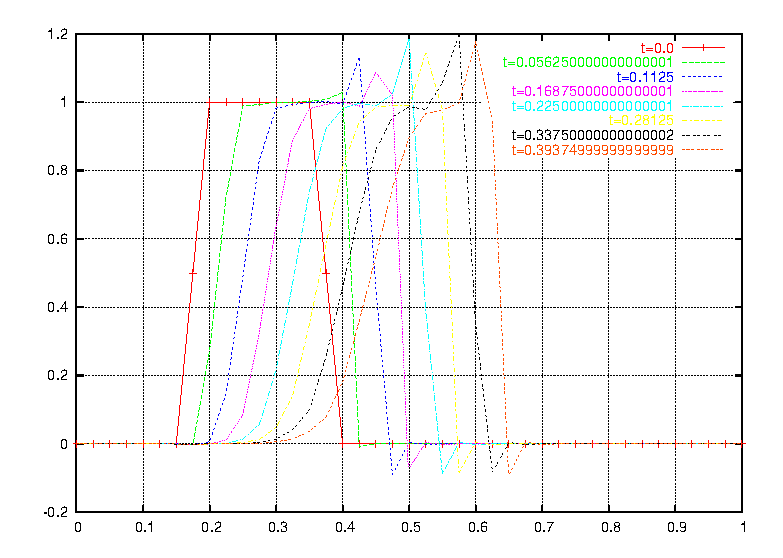
\epsfig{file=fr40.eps}
% \end{figure}
% \begin{figure}
% \caption{Pe=12.5}
% 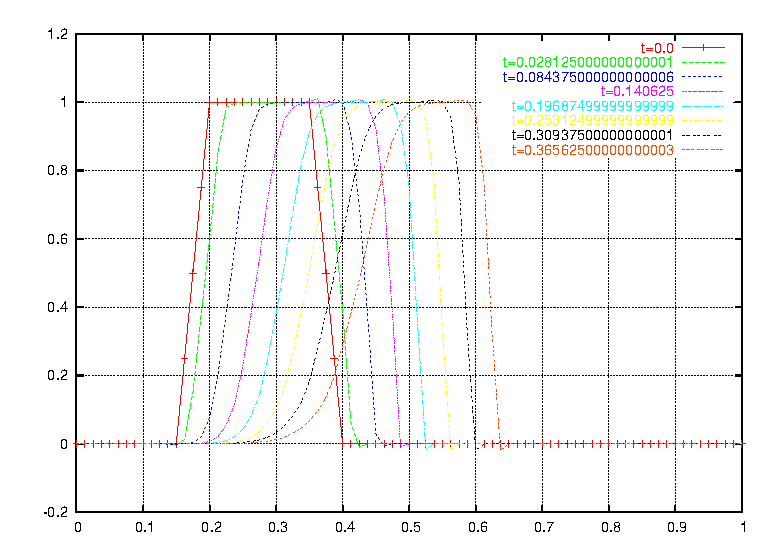
\epsfig{file=fr80.eps}
% \end{figure}
% \begin{figure}
% \caption{Pe=6}
% 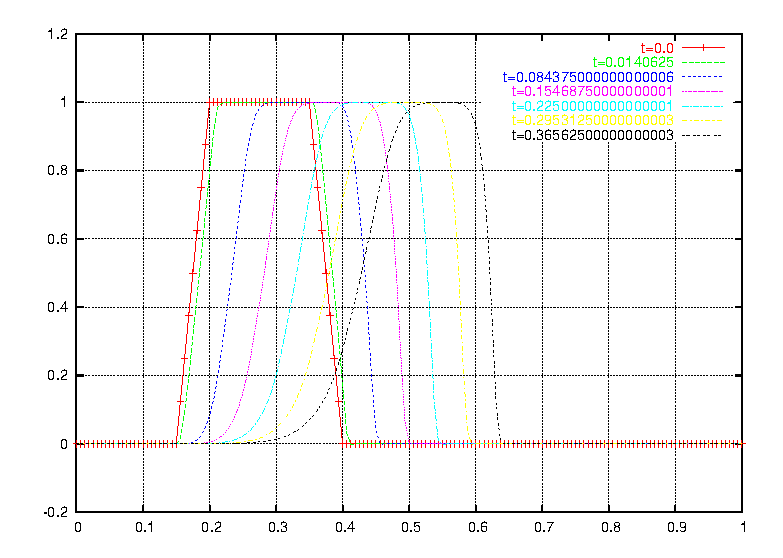
\epsfig{file=fr160.eps}
% \end{figure}

% \subsection{Local Discontinuous Galerkin}

% As a test problem for  we'll solve
% \begin{equation}
% m_t + (f - a u_x)_x = 0
% \end{equation}
% With initial-boundary conditions tba. We write this equation as a first order system
% \begin{eqnarray}
% m_t + (f - \sqrt(a) q)_x &=& 0\\
% q  - g_x &=& 0 \\
% g &=& \int^u \sqrt{a(s)} ds\\
% \end{eqnarray}
% If we let $\vec u =[u,q]'$, $\vec M(\vec u) =[m(u),0]'$ and $\vec h(\vec u) = [h_u,h_q] = [f - \sqrt{a} q,-g]'$ we have simply
% \begin{equation}
% M_t + \vec h_x =0
% \end{equation}
% To get the weak formulation we multiply by a smooth (on I) test
% function $\vec v=[v_u,v_q]'$ (componentwise multiplication $*$ )and
% integrate over some spatial domain $I=[x_{j+1/2},x_{j-1/2}]$
% \begin{equation}
% \int_I [\vec M(u)]_t * \vec v dx + \int_I [\vec h(u)]_x * \vec v dx=0
% \end{equation}
% and integrate by parts
% \begin{equation}
% \int_I [\vec M(u)]_t * \vec v dx - \int_I [\vec h(u)] * \vec v_x dx
% +\vec h( \vec u(x^-_{j+1/2})) * \vec v(x^-_{j+1/2}) -\vec h( \vec u(x^+_{j-1/2})) * \vec v(x^+_{j-1/2}) = 0 
% \end{equation}
% where $^+$ and $^-$ are the right and left limits.
% To discretize we assume we have a partition of the domain $[0,1]$
% given by ${x_{j+1/2}}_j=0^N$ and we use the weak formulation over the
% domains $I_j=(x_{j-1/2},x_{j+1/2})$ with the components of the test
% and basis functions $\vec u_h, \vec v_h$ taken from the space
% \begin{equation}
% V_h = \{ v \in L^1(0,1): v|_{I_j} \in P^k(I_j),j=1,\ldots,N \}
% \end{equation}
% Since the basis and test functions are discontinuous, the semidiscrete
% formulations using these functions will not conserve mass globally
% unless we require that $\vec h( \vec u(x^+_{j-1/2})) = \vec h( \vec
% u(x^-_{j-1/2}))$ (i.e. that the fluxes are continuous). To fulfill this
% requirement we define the numerical flux as some function $\hat{\vec
%   h}[\vec u(x^+_{j-1/2}),\vec u(x^-_{j-1/2})]$ to be specified later.
% With these definitions we obtain the finite dimensional semi-discrete weak formulation: Find $\vec u_h$ such that
% \begin{eqnarray}
% &\int_{I_j} [\vec M(\vec u_h)]_t * \vec v_h dx - \int_{I_j} [\vec h(\vec u_h)] * \vec v_{hx} dx
% +&\\
% &\hat{\vec h}[\vec u(x^+_{j+1/2}),\vec u(x^-_{j+1/2})]* \vec v_h(x^-_{j+1/2}) &\\
% &-\hat{\vec h}[\vec u(x^+_{j-1/2}),\vec u(x^-_{j-1/2})]* \vec v_h(x^+_{j-1/2}) = 0 &
% \end{eqnarray}
% for $j=0,\ldots,N$, $\forall v_h \in V_h$. The basis for $V_h$ that we
% will use will be $\{1,\frac{x-x_j}{\Delta x_j} \}$ where $x_j =
% \frac{x_{j-1/2}+x_{j+1/2}}{2}$ and $\Delta x_j=x_{j+1/2}-x_{j-1/2}$.
% The degrees of freedom for each component are then $\{v, \vec v_x\}$
% To complete the discretization we need to define the numerical flux. First we define the standard notation for averages and jumps:
% \begin{eqnarray}
% [p]&=&p^+ -  p^- \\
% \bar{p} &=& \frac{1}{2} (p^+ + p^-) \\
% \end{eqnarray}
% We define the integral transform of the flux function as we did with the square of the diffusion coefficient above:
% \begin{equation}
% \phi = \int_0^u f(s) ds 
% \end{equation}
% Now we define the numerical flux as
% \begin{equation}
% \hat{\vec h} = 
% \left\{
% \begin{array}{c}
% \frac{ \left[ \phi \right] }{ \left[ u \right] } - \frac{ \left[ g(u) \right] }{ \left[ u \right] } \bar{q} \\
% - \bar{g(u)} 
% \end{array}
% \right\}
% - \vec C 
% \left\{
% \begin{array}{c}
% \left[ u \right] \\
% \left[ q \right] 
% \end{array}
% \right\}
% \end{equation}
% The actual entries of C will determine numerical flux. We let
% \begin{equation}
% \vec C = \left\{
% \begin{array}{cc}
% \frac{|f'(u)|}{2} & -\frac{\sqrt{D(u)}}{2} \\
% \frac{\sqrt{D(u)}}{2} & 0 
% \end{array}
% \right\}
% \end{equation}
% For the case $f(u) = c$, $D(u)=a$ (linear advection/diffusion)
% \begin{equation}
% \hat{\vec h} = 
% \left\{
% \begin{array}{c}
% \frac{c}{2} (u^+ + u^-)  - \frac{\sqrt{a}}{2} (q^+ + q^-)\\
% - \frac{\sqrt{a}}{2}(u^+ + u^-) 
% \end{array}
% \right\}
% -  \left\{
% \begin{array}{c}
% \frac{|c|}{2}(u^+ - u^-) - \frac{\sqrt{a}}{2}(q^+ - q^-) \\
% \frac{\sqrt{a}}{2}(u^+ - u^-)
% \end{array}
% \right\}
% \end{equation}
% This is upwinding for the advection and supposedly the standard 3
% point stencil for diffusion if we use $P^0$ elements.

% \subsection{Implementation}
% We begin with the general ADR system
% \begin{equation}
%   \label{eq:nladrsysImp}
%   \pd{m^i}{t} + \deld \sbl \vec f^i - \sum_{j=1}^{n_c} \ten{a}^{ij} \grad \phi^j \sbr + c^i = s^i \mbox{ in } (0,T] \times U \mbox{ for } i=1,\ldots, n_c
% \end{equation}
% which we write as an abstract evolution equation on some space $X$:
% \begin{equation}
%   \label{eq:abstractEvolve}
%   \od{m^i}{t} = F^i \mbox{ for } i=1,\ldots, n_c
% \end{equation}
% where $m^i$ and $F^i$ are possibly nonlinear differential operators on
% the solution $(u^1,\ldots,u^{n_c})$. We consider linear multistep,
% Runge-Kutta, and Rosenbrock methods for the discretization of this
% problem.  Multistep methods take the form
% \begin{equation}
%   \label{eq:multistep}
%   \sum_{j=1}^{n_s} a_j m(u_{n-j}) = \sum_{j=1}^{n_s} b_j F_{n-j}(t_{n-j},u_{n-j})
% \end{equation}
% where we have dropped the component superscript $i$ and interpret the
% \eqn{multistep} as a system. Note that if $b_0 = 0$ then the method is
% semi-explit for our problem. It would still remain to solve for $u$
% based on the relation between $u$ and $m$, which is usually easy or
% even completely trivial. To put the resulting equation into focus we write it in the simpler form
% \begin{equation}
%   \label{eq:multistepReduced}
%   a_0 m_n - b_n F_n - \beta = 0
% \end{equation}

% The Runge-Kutta methods generally take the form
% \begin{eqnarray}
%   \label{eq:rungeKutta}
%   m(u_{n+1}) &=& m_n + h \sum_{j=1}^{n_s} b_j F(t_n + c_j h,u_{nj}) \\
%   m(u_{nk})  &=& m_n + h \sum_{j=1}^{n_s} a_{kj} F(t_n + c_j h,u_{nj}) 
% \end{eqnarray}

% Note that these equations represent an implicit system for
% $u_{n+1},u_{n1},\ldots, u_{ns}$. If $a_{kj} = 0$ for $k>j$ then we can
% solve this system sequentially so that that the solution can be
% obtained in $n_s$ steps where a system of the same size as the
% original PDE is solved at each stage. These are called diagonally
% implicit methods (DIRK). Furtheremore if additionally $a_{kk} = 0$
% then $m(u_{nk})$ is determined explicitly and only $m(u)$ need be
% inverted to obtain $u_{nk}$. Such a method would correspond to explit
% RK methods if $m=u$. Typically the implicit system in DIRKs is solved
% using Newton's method. The idea behind Rosenbrock methods is to
% approximate the intermediate stages using one Newton step. These
% yields methods that are linearly implicit: for our problems the
% require the solution of a linear PDE at each step rather than a
% nonlinear PDE. If we write the RK method for a diagonally implicit
% method as
% \begin{eqnarray}
%   \label{eq:rungeKutta}
%   m(u_{n+1}) &=& m_n + h \sum_{j=1}^{n_s} b_j F(t_n + c_j h,u_{nj}) \\
%   m(u_{nk})  &=& m_n + h \sum_{j=1}^{k} a_{kj} F(t_n + c_j h,u_{nj}) 
% \end{eqnarray}
% then the newton step for each stage takes the form
\bibliographystyle{plainnat} \bibliography{mp}
\end{document}








